\PassOptionsToPackage{unicode=true}{hyperref} % options for packages loaded elsewhere
\PassOptionsToPackage{hyphens}{url}
%
\documentclass[10pt,american,ignorenonframetext,aspectratio=1610]{beamer}
\RequirePackage{multicol}
\usepackage{pgfpages}
\setbeamertemplate{caption}[numbered]
\setbeamertemplate{caption label separator}{: }
\setbeamercolor{caption name}{fg=normal text.fg}
\beamertemplatenavigationsymbolsempty
% Prevent slide breaks in the middle of a paragraph:
\widowpenalties 1 10000
\raggedbottom
\setbeamertemplate{part page}{
\centering
\begin{beamercolorbox}[sep=16pt,center]{part title}
  \usebeamerfont{part title}\insertpart\par
\end{beamercolorbox}
}
\setbeamertemplate{section page}{
\centering
\begin{beamercolorbox}[sep=12pt,center]{part title}
  \usebeamerfont{section title}\insertsection\par
\end{beamercolorbox}
}
\setbeamertemplate{subsection page}{
\centering
\begin{beamercolorbox}[sep=8pt,center]{part title}
  \usebeamerfont{subsection title}\insertsubsection\par
\end{beamercolorbox}
}
\AtBeginPart{
  \frame{\partpage}
}
\AtBeginSection{
  \ifbibliography
  \else
    \frame{\sectionpage}
  \fi
}
\usepackage{lmodern}
\usepackage{amssymb,amsmath}
\usepackage{ifxetex,ifluatex}
\usepackage{fixltx2e} % provides \textsubscript
\ifnum 0\ifxetex 1\fi\ifluatex 1\fi=0 % if pdftex
  \usepackage[T1]{fontenc}
  \usepackage[utf8]{inputenc}
  \usepackage{textcomp} % provides euro and other symbols
\else % if luatex or xelatex
  \usepackage{unicode-math}
  \defaultfontfeatures{Ligatures=TeX,Scale=MatchLowercase}
\fi
\usetheme[]{Warsaw}
% use upquote if available, for straight quotes in verbatim environments
\IfFileExists{upquote.sty}{\usepackage{upquote}}{}
% use microtype if available
\IfFileExists{microtype.sty}{%
\usepackage[]{microtype}
\UseMicrotypeSet[protrusion]{basicmath} % disable protrusion for tt fonts
}{}
\IfFileExists{parskip.sty}{%
\usepackage{parskip}
}{% else
\setlength{\parindent}{0pt}
\setlength{\parskip}{6pt plus 2pt minus 1pt}
}
\usepackage{hyperref}
\hypersetup{
            pdftitle={A bio-inspired geometric model for sound reconstruction},
            pdfauthor={Rand Asswad},
            pdfborder={0 0 0},
            breaklinks=true}
\urlstyle{same}  % don't use monospace font for urls
\newif\ifbibliography
\usepackage{graphicx,grffile}
\makeatletter
\def\maxwidth{\ifdim\Gin@nat@width>\linewidth\linewidth\else\Gin@nat@width\fi}
\def\maxheight{\ifdim\Gin@nat@height>\textheight\textheight\else\Gin@nat@height\fi}
\makeatother
% Scale images if necessary, so that they will not overflow the page
% margins by default, and it is still possible to overwrite the defaults
% using explicit options in \includegraphics[width, height, ...]{}
\setkeys{Gin}{width=\maxwidth,height=\maxheight,keepaspectratio}
\setlength{\emergencystretch}{3em}  % prevent overfull lines
\providecommand{\tightlist}{%
  \setlength{\itemsep}{0pt}\setlength{\parskip}{0pt}}
\setcounter{secnumdepth}{0}

% set default figure placement to htbp
\makeatletter
\def\fps@figure{htbp}
\makeatother

\usepackage[defaultlines=10,all]{nowidow}
\usepackage{float}
\usepackage[justification=centering]{caption}
\usepackage{subcaption}

\usepackage{array}

% title frame logo

\institute{
    \begin{center}
        \centering
        \begin{minipage}[t]{0.45\textwidth}
        \raggedright
\includegraphics[height=1.5cm]{img/logo_insa.png}\\
        \textit{Department of Applied Mathematics}\\
        Natalie FORTIER\\
        Cecilia ZANNI-MERK
        \end{minipage}~\hfill~%
        \begin{minipage}[t]{0.45\textwidth}
        \raggedleft
\includegraphics[height=1.5cm]{img/logo_l2s.png}\\
        Dario PRANDI\\
        Ugo BOSCAIN
        \end{minipage}
    \end{center}
}

% beamer shit

\setbeamertemplate{footline}{
\leavevmode%
\hbox{\hspace*{-0.06cm}
\begin{beamercolorbox}[wd=.2\paperwidth,ht=2.25ex,dp=1ex,center]{author in head/foot}%
	\usebeamerfont{author in head/foot}\insertshortauthor
\end{beamercolorbox}%
\begin{beamercolorbox}[wd=.6\paperwidth,ht=2.25ex,dp=1ex,center]{section in head/foot}%
	\usebeamerfont{section in head/foot}\insertshorttitle
\end{beamercolorbox}%
\begin{beamercolorbox}[wd=.2\paperwidth,ht=2.25ex,dp=1ex,right]{section in head/foot}%
	\usebeamerfont{section in head/foot}\insertshortdate{}\hspace*{1em}
	\insertframenumber/\inserttotalframenumber\hspace*{1em}
\end{beamercolorbox}}%
\vskip0pt%
}

% theorem environments

%\theoremstyle{theorem}
\newtheorem{prop}{Proposition}[section]

\theoremstyle{remark}
\newtheorem*{remark}{Remark}

\def\R{\mathbb{R}}
\def\C{\mathbb{C}}
\def\N{\mathbb{N}}
\def\Z{\mathbb{Z}}

\def\Cl{\mathcal{C}}
\def\U{\mathcal{U}}
\def\H{\mathbb{H}}

\def\w{\omega}
\let\aphi\phi
\def\phi{\varphi}
\def\epsilon{\varepsilon}

\def\numin{\nu_{\min}}
\def\numax{\nu_{\max}}

\def\ddt{\frac{\mathrm{d}}{\mathrm{d}t}}
\def\dx{\mathrm{d}x}
\def\dt{\mathrm{d}t}
\def\ds{\mathrm{d}s}
\def\dtau{\mathrm{d}\tau}
\def\dw{\mathrm{d}\w}
\def\dnu{\mathrm{d}\nu}
\def\dtheta{\mathrm{d}\theta}
\def\dtfrac{\frac{\partial}{\partial t}}

\def\pp#1{\left(#1\right)}
\def\sset#1{\left\{#1\right\}}
\def\vset#1#2{\sset{#1\left\lvert#2\right.}}

\def\abs #1{\left\lvert#1\right\rvert}
\def\norm#1{\left\lVert#1\right\rVert}
\def\dotp#1{\left\langle#1\right\rangle}
\def\round#1{\left\lfloor#1\right\rceil}

\def\bbar#1{\overline{#1}}

\def\pmat#1{\begin{pmatrix}#1\end{pmatrix}}
\def\hmat#1#2{\pmat{#1 & #2\\0 & 1}}

\def\Aut{\mathrm{Aut}}

\def\qtext#1{\quad\text{#1}\quad}

\def\argmin{\mathop{\mathrm{argmin}}}
\def\argmax{\mathop{\mathrm{argmax}}}
\def\supp{\mathop{\mathrm{supp}}}

\def\transp#1{{#1}^{\top}}

\def\stft #1{\mathrm{STFT}\sset{#1}}
\def\STFT{\mathrm{STFT}}
\def\Proj{\mathrm{Proj}}

\def\Cd{\mathrm{Cauchy}}

\DeclareUnicodeCharacter{03BD}{$\nu$}
\ifnum 0\ifxetex 1\fi\ifluatex 1\fi=0 % if pdftex
  \usepackage[shorthands=off,main=american]{babel}
\else
  % load polyglossia as late as possible as it *could* call bidi if RTL lang (e.g. Hebrew or Arabic)
  \usepackage{polyglossia}
  \setmainlanguage[variant=american]{english}
\fi

\title{A bio-inspired geometric model for sound reconstruction}
\providecommand{\subtitle}[1]{}
\subtitle{Master's Thesis}
\author{Rand Asswad}
\date{23 September 2021}

\begin{document}
\frame[plain]{\titlepage}

\begin{frame}
\frametitle{Outline}
\begin{multicols}{2}
\tableofcontents
\end{multicols}
\end{frame}
\hypertarget{introduction}{%
\section{Introduction}\label{introduction}}

\begin{frame}{Laboratory of Signals and Systems (L2S)}
\protect\hypertarget{laboratory-of-signals-and-systems-l2s}{}

\begin{itemize}
\tightlist
\item
  Created in 1974
\item
  Affiliations:

  \begin{itemize}
  \tightlist
  \item
    CNRS (Centre National de la Recherche Scientifique)
  \item
    CentraleSupélec
  \item
    University of Paris-Saclay
  \end{itemize}
\item
  Research fields:

  \begin{itemize}
  \tightlist
  \item
    Systems and control
  \item
    Signal processing and statistics
  \item
    Networks and telecommunication
  \end{itemize}
\end{itemize}

\end{frame}

\begin{frame}{Supervision}
\protect\hypertarget{supervision}{}

\begin{itemize}
\tightlist
\item
  Dario Prandi

  \begin{itemize}
  \tightlist
  \item
    Affiliations: L2S, CNRS, CentraleSupélec, Université Paris-Saclay
  \item
    Specialties:

    \begin{itemize}
    \tightlist
    \item
      Geometric control theory
    \item
      Biomimetic image processing
    \item
      Diffusions on singular manifolds
    \end{itemize}
  \end{itemize}
\item
  Ugo Boscain

  \begin{itemize}
  \tightlist
  \item
    Affiliations: Laboratoire Jacques-Louis Lions, CNRS, Inria, Sorbonne
    Université
  \item
    Specialties:

    \begin{itemize}
    \tightlist
    \item
      Sub-riemannian geometry
    \item
      Control of quantum mechanical systems
    \item
      (also) optimal control and switched systems
    \end{itemize}
  \end{itemize}
\end{itemize}

\end{frame}

\begin{frame}[fragile]{Internship mission}
\protect\hypertarget{internship-mission}{}

Work on the proposed neuro-geometric sound reconstruction model.

Subtasks:

\begin{itemize}
\tightlist
\item
  Study the existing model
\item
  Test on real speech signals
\item
  Publish results
\item
  Reimplement \texttt{WCA1.jl} package
\item
  Rethink model \& study litterature
\end{itemize}

\end{frame}

\hypertarget{image-reconstruction-model}{%
\section{Image reconstruction model}\label{image-reconstruction-model}}

\hypertarget{neuro-geometric-model-of-v1}{%
\subsection{Neuro-geometric model of
V1}\label{neuro-geometric-model-of-v1}}

\begin{frame}{Basis of the V1 model - starting point}
\protect\hypertarget{basis-of-the-v1-model---starting-point}{}

\begin{enumerate}
\tightlist
\item
  Hubel and Weisel (1959) {[}\protect\hyperlink{ref-hubel1959}{13}{]}
  observed that there are groups of neurons sensitive to positions and
  directions
\end{enumerate}

\centering

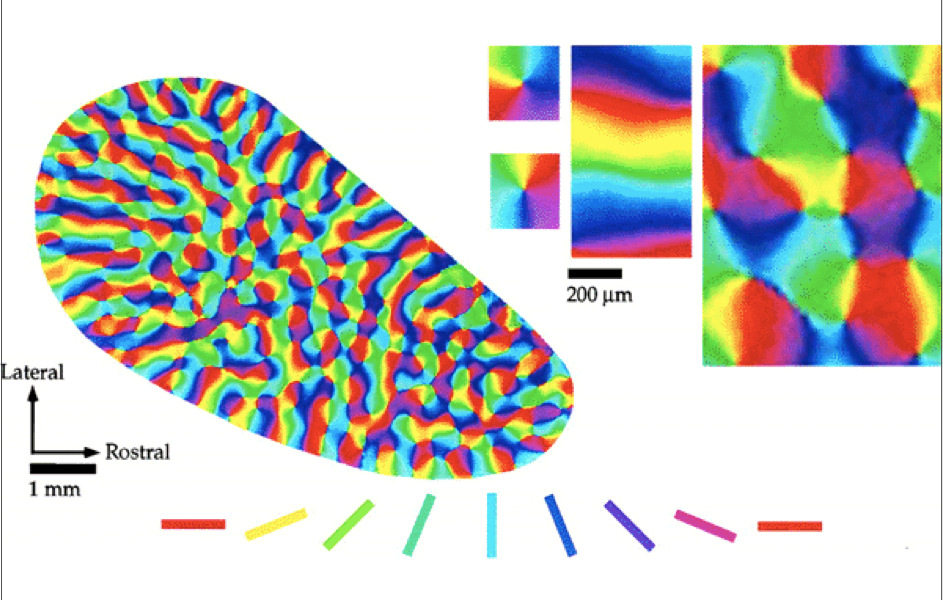
\includegraphics[width=\textwidth,height=0.65\textheight]{img/hubel1959.jpg}

\end{frame}

\begin{frame}{Basis of the V1 model - 3D representation}
\protect\hypertarget{basis-of-the-v1-model---3d-representation}{}

\begin{enumerate}
\setcounter{enumi}{1}
\tightlist
\item
  Which inspired Hoffman (1989)
  {[}\protect\hyperlink{ref-hoffman1989}{12}{]} to model V1 as a contact
  space (a 3D manifold endowed with a smooth map)
\item
  The Citti-Petitot-Sarti (CPS) model (2006)
  {[}\protect\hyperlink{ref-citti2006}{7},\protect\hyperlink{ref-petitot1999}{16}{]}
  extended the model to sub-Riemannian structures
\end{enumerate}

The CPS model:

\begin{columns}[T]
\begin{column}{0.5\textwidth}
\begin{itemize}
\item
  An image can be seen as a function \(f:\R^2\rightarrow\R_+\)
  representing the grey level at given coordinates
\item
  The primary visual cortex (V1) adds the non-directed angle
  \(\theta\in P^1=\R/\pi\Z\) of the tangent line to the curve.

  The visual cortex lifts a curve into \(\R^2\times P^1\).
\end{itemize}
\end{column}

\begin{column}{0.5\textwidth}
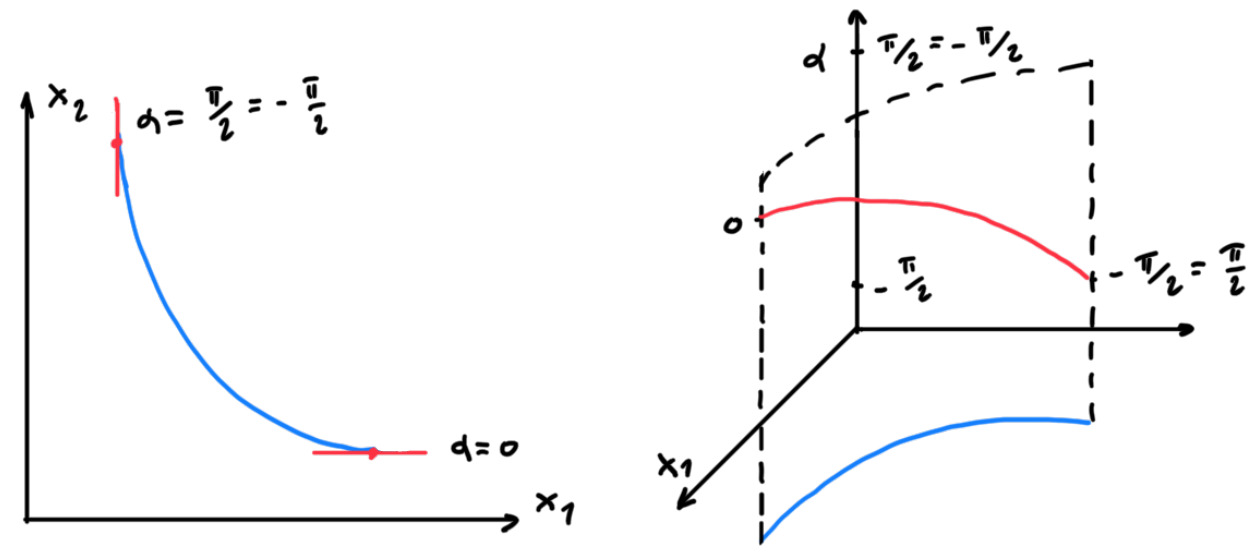
\includegraphics{img/v1_model_1.jpg}
\end{column}
\end{columns}

\end{frame}

\begin{frame}{Basis of the V1 model - image reconstruction}
\protect\hypertarget{basis-of-the-v1-model---image-reconstruction}{}

\begin{enumerate}
\setcounter{enumi}{3}
\tightlist
\item
  Ugo Boscain, Dario Prandi, Jean-Paul Gauthier, and their colleagues
  proposed (in 2017)
  {[}\protect\hyperlink{ref-bertalmio2018}{2},\protect\hyperlink{ref-boscain2017}{3}{]}
  an image reconstruction model based on the CPS model.
\end{enumerate}

If a curve is interrupted in an interval, then the visual cortex tries
to reconstruct it by taking the shortest curve in the lifted space.

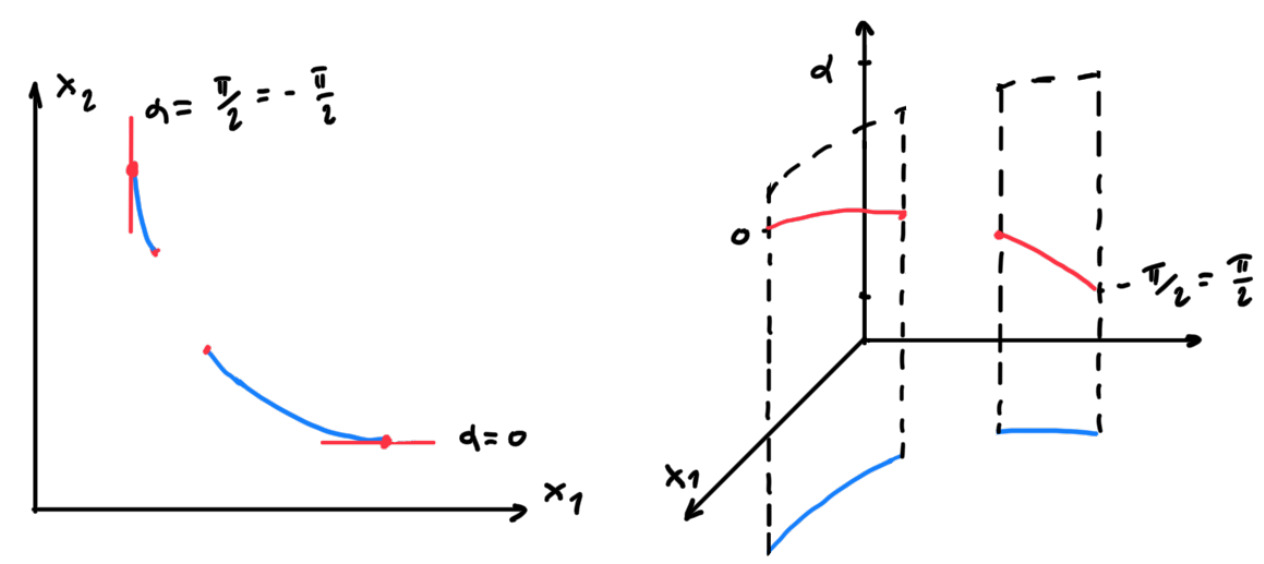
\includegraphics[width=0.7\textwidth,height=\textheight]{img/v1_model_2.jpg}

\end{frame}

\hypertarget{image-reconstruction-model-1}{%
\subsection{Image reconstruction
model}\label{image-reconstruction-model-1}}

\begin{frame}{Wilson-Cowan model
{[}\protect\hyperlink{ref-wilson1972}{19}{]}}
\protect\hypertarget{wilson-cowan-model-wilson1972}{}

\begin{itemize}
\tightlist
\item
  The Wilson-Cowan (WC) model describes the evolution of neural
  activations
\item
  WC describes the evolution of excitatory and inhibitory activity in a
  synaptically coupled neuronal network
\item
  The interaction between the hypercolumns in V1 can be described
  through the WC equation {[}\protect\hyperlink{ref-bressloff2002}{5}{]}
\end{itemize}

Let \(a(x,\theta,t)\) be the state of a population of neurons with
coordinates \(x\in\R^2\) and orientation \(\theta\in P^1\) at time
\(t>0\), the WC integro-differential equation is given by
{[}\protect\hyperlink{ref-bertalmio2018}{2}{]}

\[ \dtfrac a(x,\theta,t) = -\alpha a(x,\theta,t) + \nu
\int_{\R^2\times P^1} \omega(x,\theta\| x',\theta') \sigma(a(x',\theta',t)) \dx'\dtheta'
+ h(x,\theta,t) \]

\end{frame}

\begin{frame}{Reconstruction of a 97\% corrupted image}
\protect\hypertarget{reconstruction-of-a-97-corrupted-image}{}

\begin{columns}[T]
\begin{column}{0.3\textwidth}
\centering

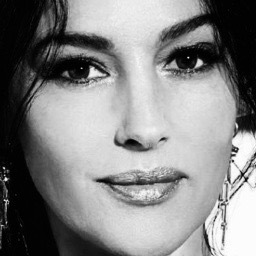
\includegraphics{img/img_original.jpg} original
\end{column}

\begin{column}{0.3\textwidth}
\centering

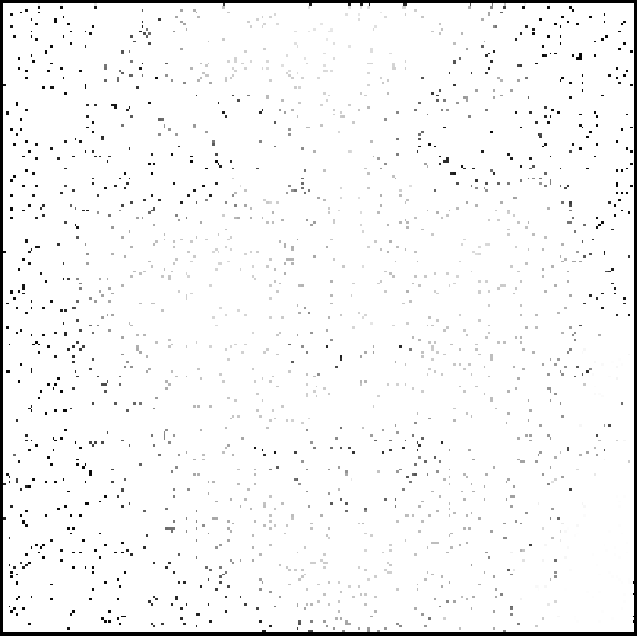
\includegraphics{img/img_corrupted.png} corrupted
\end{column}

\begin{column}{0.3\textwidth}
\centering

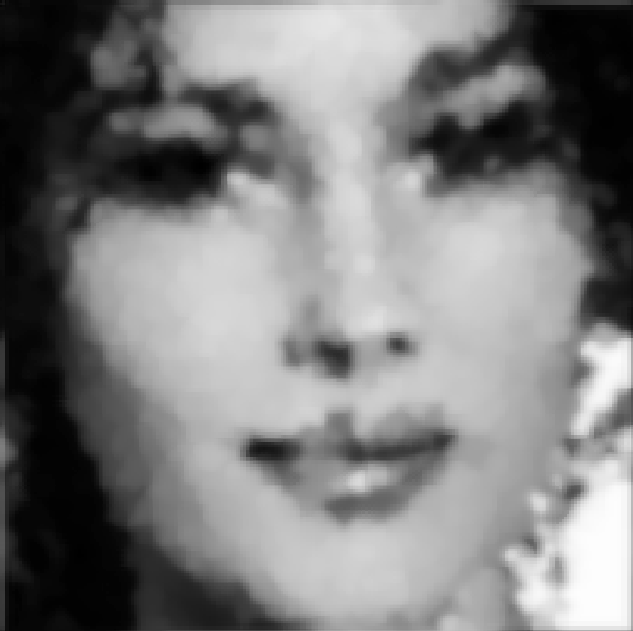
\includegraphics{img/img_reconstructed.png} reconstructed
\end{column}
\end{columns}

\end{frame}

\begin{frame}{Which begs the question}
\protect\hypertarget{which-begs-the-question}{}

Can we apply these ideas to the problem of sound reconstruction?

\end{frame}

\hypertarget{sound-reconstruction-model}{%
\section{Sound reconstruction model}\label{sound-reconstruction-model}}

\hypertarget{from-v1-to-a1}{%
\subsection{From V1 to A1}\label{from-v1-to-a1}}

\begin{frame}{Motivation}
\protect\hypertarget{motivation}{}

A sound signal \(s(t)\) can be seen as an image in the time-frequency
domain \(|S|(\tau,\w)\)

\centering

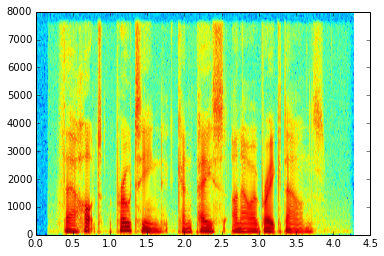
\includegraphics[height=.7\textheight]{img/speech_spectrum.png}

\end{frame}

\begin{frame}{Taking into account:}
\protect\hypertarget{taking-into-account}{}

\begin{enumerate}
\tightlist
\item
  In image reconstruction the whole image is evolved simultaneously.
  However, the sound image (spectrogram) does not reach the auditory
  cortex simultaneously but \emph{sequentially}. Hence, the
  reconstruction can be performed only in a sliding window.
\item
  A rotated sound image corresponds to a completely different input
  sound, therefore the invariance by rototranslation is lost.
\end{enumerate}

\end{frame}

\begin{frame}{Sound signal processing in the cochlea}
\protect\hypertarget{sound-signal-processing-in-the-cochlea}{}

\begin{columns}[T]
\begin{column}{0.7\textwidth}
The primary auditory cortex (A1) receives the sensory input directly
from the cochlea {[}\protect\hyperlink{ref-dallos1996}{8}{]}, which is a
spiral-shaped fluid-filled cavity that composes the inner ear.

\begin{itemize}
\tightlist
\item
  The mechanical vibrations along the basilar membrane are transduced
  into electrical activity along a dense, topographically ordered, array
  of auditory-nerve fibers (hair cells) which convey these electrical
  potentials to the central auditory system.
\item
  Since the inner hair cells are topographically ordered along the
  cochlea spiral, different regions of the cochlea are sensitive to
  frequencies as follows {[}\protect\hyperlink{ref-yang1992}{20}{]}:

  \begin{itemize}
  \tightlist
  \item
    Hair cells close to the base are more sensitive to low-frequency
    sounds
  \item
    near the apex are more sensitive to high-frequency sounds
  \end{itemize}
\end{itemize}
\end{column}

\begin{column}{0.3\textwidth}
\centering

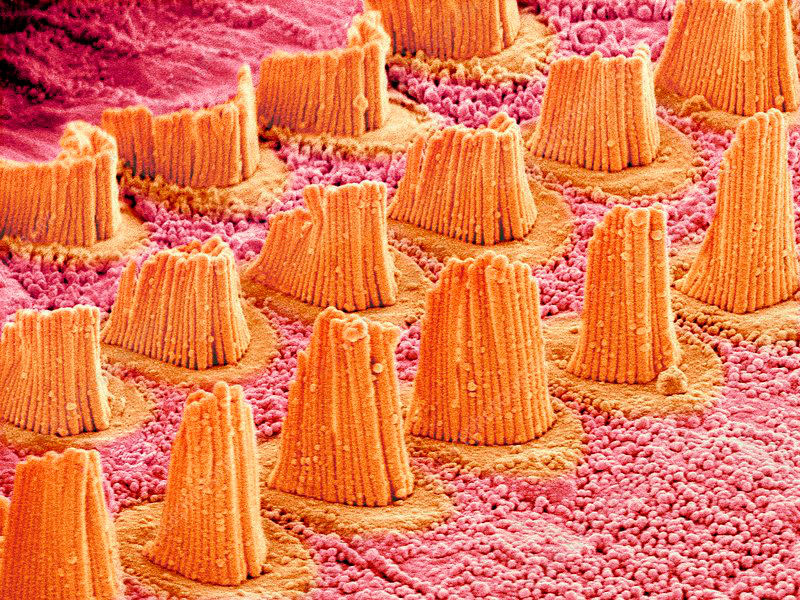
\includegraphics[width=0.8\textwidth,height=\textheight]{img/hair_cells.jpg}

\par\vspace{1em}\par

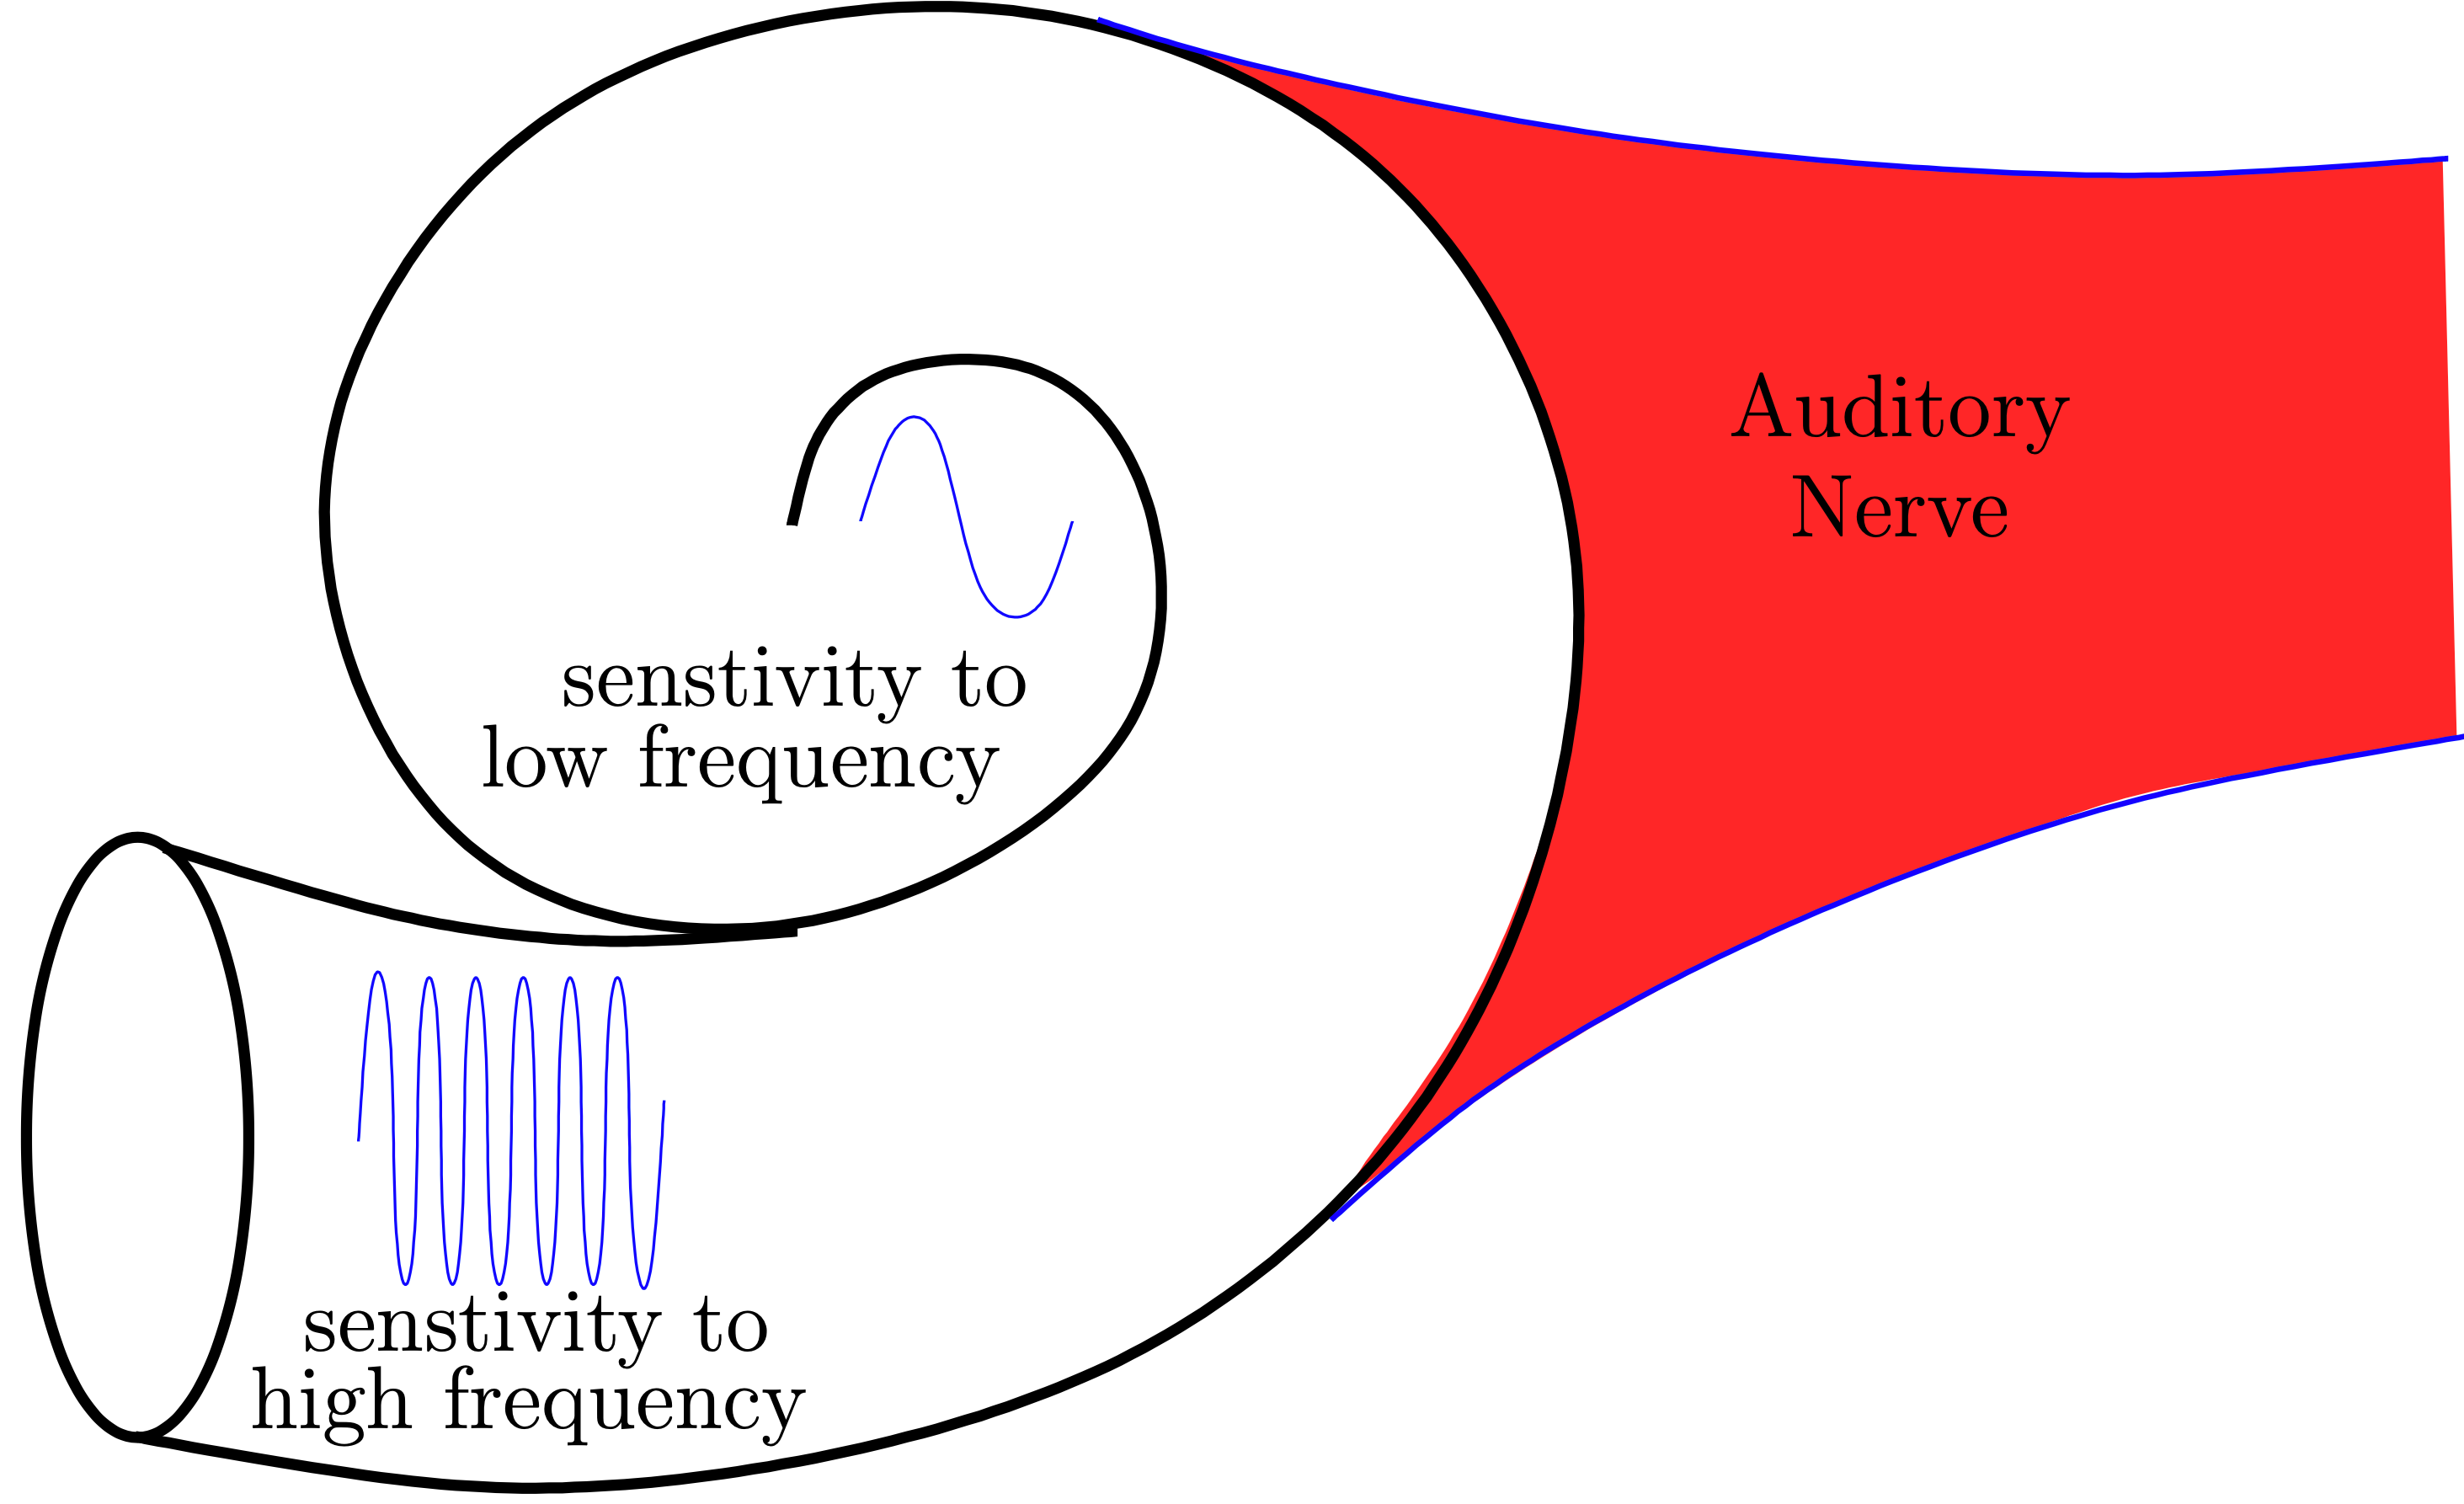
\includegraphics{img/cochlea.png}
\end{column}
\end{columns}

\end{frame}

\begin{frame}{Sound reconstruction pipeline}
\protect\hypertarget{sound-reconstruction-pipeline}{}

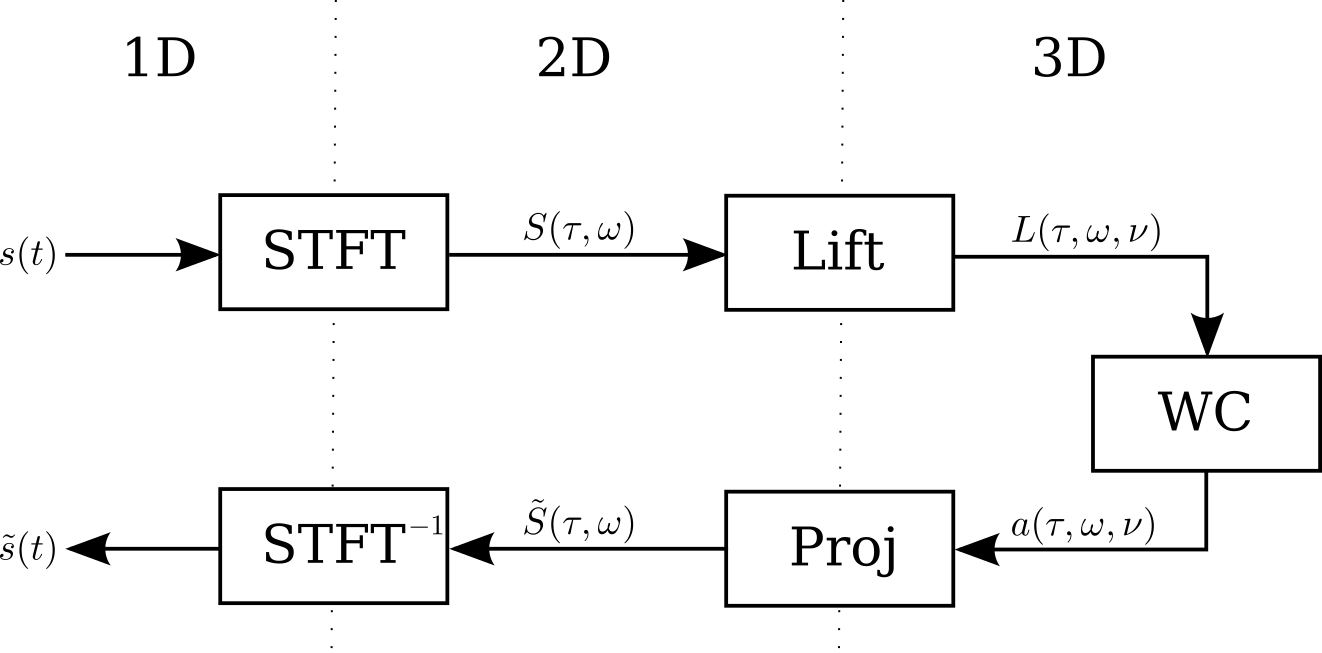
\includegraphics[width=1\textwidth,height=\textheight]{img/pipeline.png}

\end{frame}

\hypertarget{time-frequency-representation}{%
\subsection{Time-Frequency
representation}\label{time-frequency-representation}}

\begin{frame}{Time representation \& Frequency representation}
\protect\hypertarget{time-representation-frequency-representation}{}

\begin{columns}[T]
\begin{column}{0.6\textwidth}
We consider a realizable sound signal \(s\in L^2(\R)\)

\begin{itemize}
\tightlist
\item
  \textbf{Frequency representation:}
  \[\hat s(\w) = \F\sset{s(t)}(\w) = \int_\R s(t) e^{-2\pi i\w t}\dt\]
\item
  \textbf{Time representation:}
  \[s(t) = \F^{-1}\sset{\hat s(\w)}(t) = \int_\R \hat s(\w) e^{2\pi i\w t}\dw\]
\end{itemize}

Since \(s=\F^{-1}\sset{\hat s}\), we can say about \(s\) and \(\hat s\)
that they

\begin{itemize}
\tightlist
\item
  both contain the exact same information
\item
  both represent the same object \(s\in L^2(\R)\)
\item
  they simply show different features of \(s\)
\end{itemize}
\end{column}

\begin{column}{0.4\textwidth}
\centering

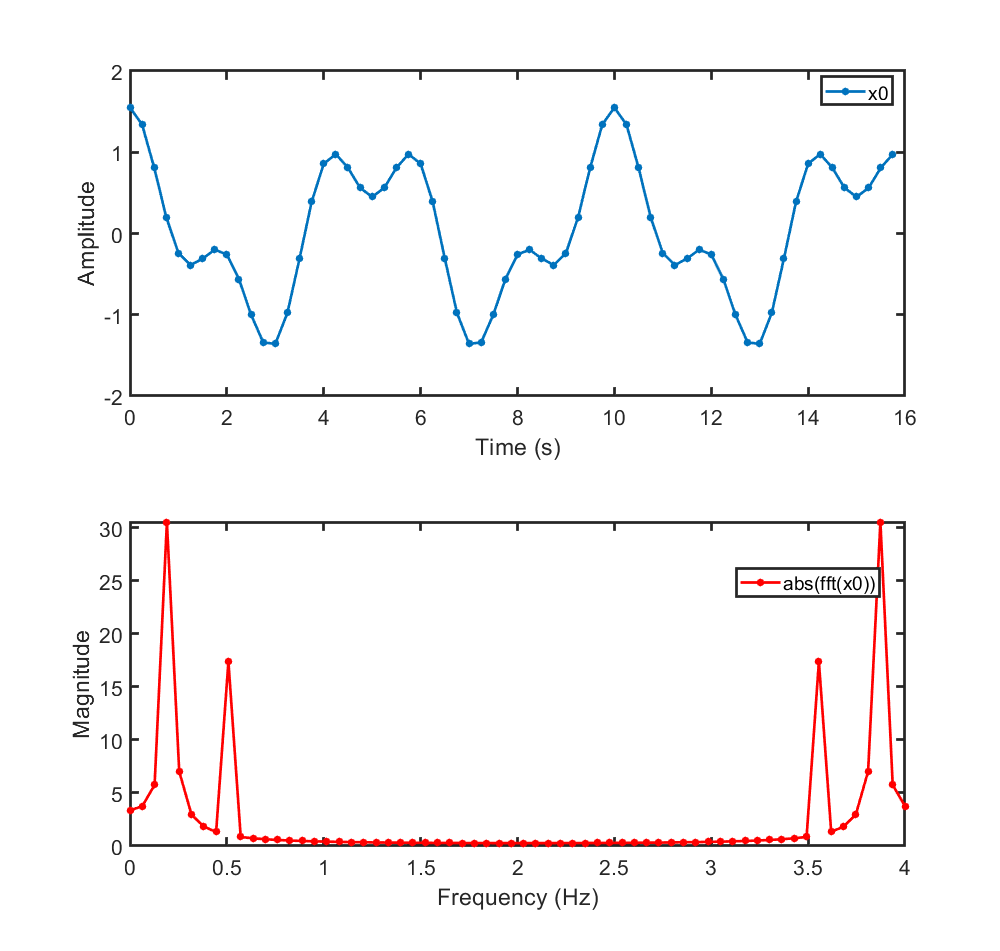
\includegraphics{img/signal_vs_spectrum.png}
\end{column}
\end{columns}

A time-frequency representation would combine the features of both \(s\)
and \(\hat s\) into a single function. Such representation provides an
\emph{instantaneous frequency spectrum} of the signal at any given time
{[}\protect\hyperlink{ref-grochenig2001}{11}{]}.

\end{frame}

\begin{frame}{Short-Time Fourier Transform (STFT)}
\protect\hypertarget{short-time-fourier-transform-stft}{}

\begin{definition}[Short-Time Fourier Transform]
Let $s\in L^2(\R)$ be a time signal, let $\w\in L^2(\R)$ be a compactly supported window
centered around $0$.
The STFT of $s$ with respect to the window $w$ is defined as
$$S(\tau,\w) = \stft{s(t)}(\tau,\w) = \int_\R s(t)w(t-\tau)e^{-2\pi i\w t} \dt$$
\end{definition}

\begin{columns}[T]
\begin{column}{0.6\textwidth}
The STFT is

\begin{itemize}
\tightlist
\item
  a very common time-frequency representation of a signal
\item
  the Fourier transform of the \(s(t)w(t-\tau)\), the signal taken over
  a sliding window along the time axis
\item
  usually taken along a smooth window because a sharp cut-off introduces
  discontinuities and aliasing issues
  {[}\protect\hyperlink{ref-grochenig2001}{11}{]}
\end{itemize}
\end{column}

\begin{column}{0.4\textwidth}
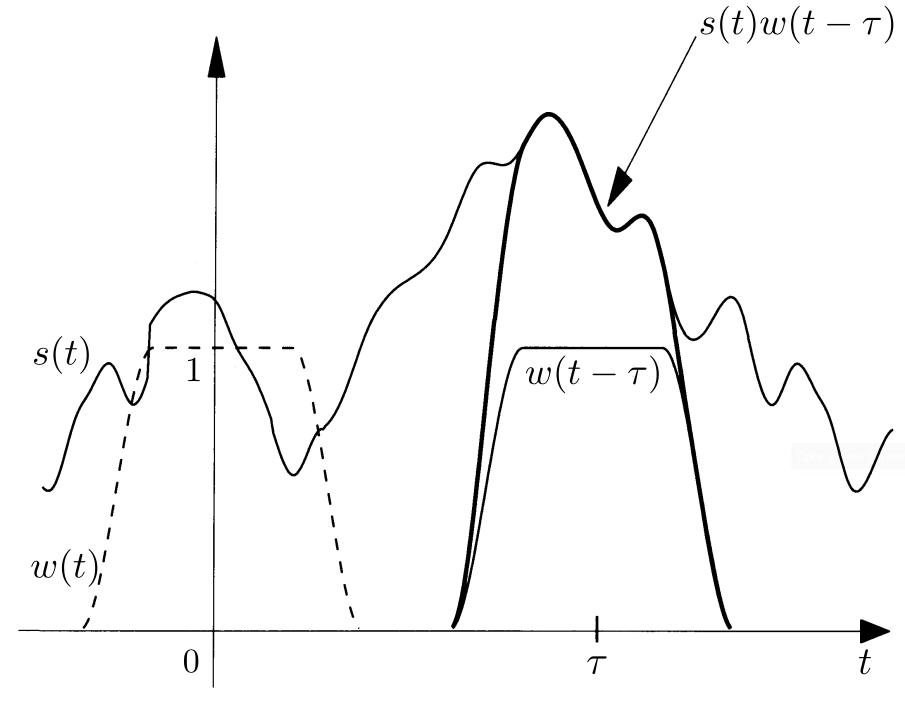
\includegraphics{img/stft_grochenig.png}
\end{column}
\end{columns}

\end{frame}

\begin{frame}{Time and frequency shifts operators}
\protect\hypertarget{time-and-frequency-shifts-operators}{}

\begin{definition}[Time and frequency shifts operators]
Let $s\in L^2(\R)$ be a time signal, we define for all $\tau,\w\in\R$
\begin{itemize}
  \item \textbf{Time shift operator:}  $T_\tau s(t)=s(t-\tau)$
  \item \textbf{Phase shift operator:} $M_\w s(t)=e^{2\pi i \w t} s(t)$
\end{itemize}
We call $T_\tau$ and $M_\w$ unitary operators in $\U(L^2(\R))$
\end{definition}

The STFT can be formulated using these unitary operators \begin{align*}
S(\tau,\w) &= \int_\R s(t)w(t-\tau)e^{-2\pi i\w t} \dt\\
    &= \int_\R s(t) \overline{M_\w T_\tau w(t)} \dt\\
    &= \dotp{s, M_\w T_\tau w}_{L^2(\R)}
\end{align*}

We can redefine the STFT as an operator \(V_w\) on \(s\in L^2(\R)\)
defined in function of \(T_\tau,M_\w\in\U(L^2(\R))\)
{[}\protect\hyperlink{ref-boscain2021}{4},\protect\hyperlink{ref-grochenig2001}{11}{]}.
\[V_w s(\tau,\w) = \dotp{s, M_\w T_\tau w}_{L^2(\R)}\]

\end{frame}

\begin{frame}{Discrete STFT}
\protect\hypertarget{discrete-stft}{}

Similarly to the continuous STFT, the discrete STFT is the Discrete
Fourier Transform (DFT) of the signal over a sliding window.
Nevertheless, the window cannot slide continuously along the time axis,
instead the signal is windowed at different frames with an overlap. The
window therefore hops along the time axis.

Discrete STFT parameters:

\begin{itemize}
\tightlist
\item
  Window size (DFT size): \(N\)
\item
  Overlap size: \(R\)
\item
  Hop size: \(H=N-R\)
\item
  Overlap ratio: \(r=R/N\in[0,1[\)
\end{itemize}

\begin{definition}[Discrete Short-Time Fourier Transform]
The discrete STFT of a signal $s\in L^2([0,T])$ over a window $w$ is defined as
$$S[m,\w] = \sum_{t=0}^{T} s[t]w[t-mH]e^{-2\pi i\w t}$$
\end{definition}

\end{frame}

\begin{frame}{STFT windowing}
\protect\hypertarget{stft-windowing}{}

The choice of the window affects the quality of the Fourier transform.

\begin{tabular}{ >{\centering\arraybackslash} m{3cm} >{\centering\arraybackslash} m{9cm} }

Window function & $\hspace{.7cm}s(t)w(t-t_0) \hspace{1.7cm} \F\sset{s(t)w(t-t_0)}(\w)$\\\hline
Rectangular     & 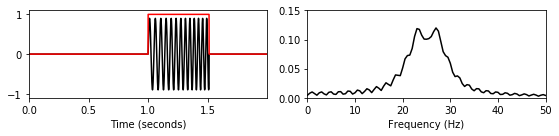
\includegraphics[width=.6\textwidth]{img/w_rectangle.png}\\
Triangular      & 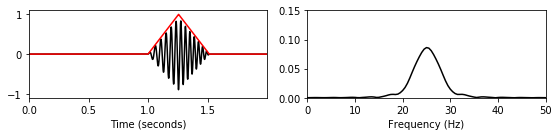
\includegraphics[width=.6\textwidth]{img/w_triangle.png}\\
Hann            & 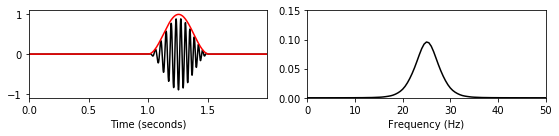
\includegraphics[width=.6\textwidth]{img/w_hann.png}
\end{tabular}

\end{frame}

\begin{frame}{STFT windowing - invertibility constraints}
\protect\hypertarget{stft-windowing---invertibility-constraints}{}

\begin{columns}[T]
\begin{column}{0.6\textwidth}
The STFT is invertible if its parameters satisfy the two following
constraints
{[}\protect\hyperlink{ref-griffin1983}{10},\protect\hyperlink{ref-muller2015}{15}{]}:

\begin{itemize}
\tightlist
\item
  \textbf{Nonzero OverLap Add (NOLA):}
  \[\sum\limits_{m\in\Z} w^2[t-mH] \neq 0\]
\item
  \textbf{Constant OverLap Add (COLA):}
  \[\sum\limits_{m\in\Z} w[t-mH] = 1\]
\end{itemize}
\end{column}

\begin{column}{0.4\textwidth}
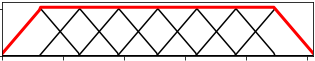
\includegraphics[width=\textwidth]{img/woa_triangular_1_2.png}

\par

Triangular window, overlap ratio \(r=\frac{1}{2}\)
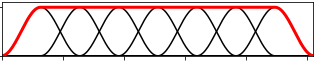
\includegraphics[width=\textwidth]{img/woa_hann_1_2.png}

\par

Hann window, overlap ratio \(r=\frac{1}{2}\)
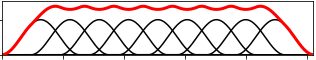
\includegraphics[width=\textwidth]{img/woa_hann_3_8.png}

\par

Hann window, overlap ratio \(r=\frac{3}{8}\)
\end{column}
\end{columns}

The NOLA condition is met for any window given an overlap ratio
\(r\in[0,1[\). It is worth noting that this condition can be found
without the square depending on the inverse STFT algorithm.

The COLA constraint defines the partition of unity over the discrete
time axis, imposing a stronger condition.

\end{frame}

\begin{frame}{STFT windowing - Hann window}
\protect\hypertarget{stft-windowing---hann-window}{}

\begin{remark}
In typical applications, the window functions used are non-negative,
smooth, bell-shaped curves.
\end{remark}

In our model we use the Hann window, which satisfies the COLA condition
for any overlap ratio of \(r=\frac{n}{n+1},n\in\N^*\).

The Hann window of length \(L\) is defined as \[w(x)=\begin{cases}
\frac{1+\cos\pp{\frac{2\pi x}{L}}}{2} & \text{if}~\abs{x}\leq\frac{L}{2}\\
0 & \text{if}~\abs{x}>\frac{L}{2}
\end{cases}\]

\end{frame}

\begin{frame}{Uncertainty principles}
\protect\hypertarget{uncertainty-principles}{}

In mathematics, uncertainty principles are

\begin{itemize}
\tightlist
\item
  limits to the accuracy with which the values for certain physical
  pairs can be obeserved
\item
  inequilities that involve pairs of complementary/disjoint variables
\end{itemize}

Common examples are

\begin{itemize}
\tightlist
\item
  \textbf{Heisenberg's Uncertainty Principle:} a particle's momentum and
  its position
\item
  \textbf{The Heisenberg-Gabor limit:} a signal's time and frequency
\end{itemize}

\begin{theorem}[Heisenberg-Pauli-Weyl inequality]
Let $f\in L^2(\R)$, then $\forall a,b\in\R$
$$ \pp{\int_\R (t-a)^2\abs{f(t)}^2\dt}^{1/2}
   \pp{\int_\R (\w-b)^2\abs{\hat f(\w)}^2\dw}^{1/2}
   \geq \frac{\norm{f}_2^2}{4\pi}$$
\end{theorem}

\end{frame}

\begin{frame}{Uncertainty principle - the Heisenberg-Gabor limit}
\protect\hypertarget{uncertainty-principle---the-heisenberg-gabor-limit}{}

From the Heisenberg-Pauli-Weyl Inequality, we obtain the following
theorem

\begin{theorem}[Heisenberg-Gabor limit]
Let $f\in L^2(\R)$, if $\norm{f}_2 = 1$ then
$$\sigma_t\cdot\sigma_\w \geq \frac{1}{4\pi}$$
where $\sigma_t$ and $\sigma_\w$ are the standard deviations of the time and frequency respectively.
\end{theorem}

Interpretation of the standard deviations:

\begin{itemize}
\tightlist
\item
  \(\sigma_t\) is the size of the \emph{essential support} of \(f\)
\item
  \(\sigma_\w\) is the size of the \emph{essential bandwidth} of the
  signal centered around the average frequency \(\bar\w\)
\end{itemize}

The Gabor limit means that

\begin{itemize}
\tightlist
\item
  ``a realizable signal occupies a region of area at least one in the
  time-frequency plane.''
\item
  we cannot sharply localize a signal in both the time domain and
  frequency domain
\item
  the concept of an instantaneous frequency is impossible
  {[}\protect\hyperlink{ref-grochenig2001}{11}{]}
\end{itemize}

\end{frame}

\begin{frame}{Uncertainty principle - resolution issues}
\protect\hypertarget{uncertainty-principle---resolution-issues}{}

STFT resolution with respect to different window sizes \(\Delta T\) and
overlap ratios \(r\)

\begin{columns}[T]
\begin{column}{0.6\textwidth}
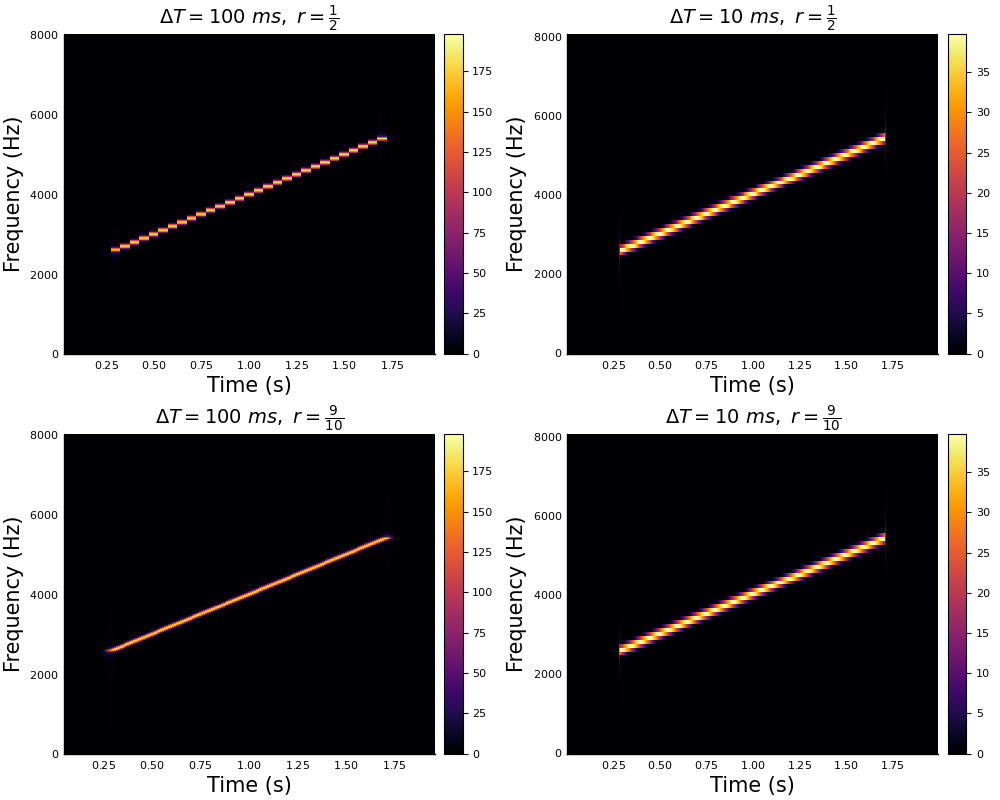
\includegraphics[width=\textwidth,height=0.8\textheight]{img/stft_resolution.png}
\end{column}

\begin{column}{0.4\textwidth}
Influence of the window size and the overlap ratio:

\begin{itemize}
\tightlist
\item
  \textbf{Window size:}

  \begin{itemize}
  \tightlist
  \item
    Larger windows \(\implies\) higher frequency resolution \& lower
    time resolution
  \item
    Smaller windows \(\implies\) lower frequency resolution \& higher
    time resolution
  \end{itemize}
\item
  \textbf{Overlap:}

  \begin{itemize}
  \tightlist
  \item
    Small overlaps \(\implies\) time discontinuities \& computationally
    cheaper
  \item
    Big overlaps \(\implies\) more time precision \& computationally
    costly
  \end{itemize}
\end{itemize}
\end{column}
\end{columns}

\end{frame}

\begin{frame}{Inverse STFT}
\protect\hypertarget{inverse-stft}{}

\begin{theorem}[Parseval's Formula for the STFT]
Consider two signals $s_1,s_2\in L^2(\R)$, and two windows $w_1,w_2\in L^2(\R)$, then
$$ \dotp{V_{w_1}s_1,V_{w_2}s_2}_{L^2(\R^2)} =
   \dotp{s_1,s_2}_{L^2(\R)} \bbar{\dotp{w_1,w_2}}_{L^2(\R)} $$
\end{theorem}

\begin{prop}
If $\norm{w}_2=1$ then the STFT operator $W_w$ is an isometry from $L^2(\R)$ to $L^2(\R^2)$.\par
This can be easily shown from Parseval's Formula
$$ \forall s,w\in L^2(\R), \norm{V_w s}_2=\norm{s}_2 \norm{w}_2\implies 
  \norm{V_w s}_2=\norm{s}_2,\forall s\in L^2(\R)~\text{if}~\norm{w}_2=1$$
\end{prop}

\begin{theorem}[Inverse Short-Time Fourier Transform]
Let $w,h\in L^2(\R)$ with $\dotp{w,h}\neq0$. Then for all $s\in L^2(\R)$
$$s(t) = \frac{1}{\dotp{w,h}} \iint_{\R^2}V_w s(\tau,\w)M_\w T_\tau h(t) \dw\dtau
       = \frac{1}{\dotp{w,h}} \iint_{\R^2} S(\tau,\w) h(t-\tau) e^{2\pi i\w t} \dw\dtau $$
\end{theorem}

\end{frame}

\begin{frame}{Inverse STFT - Griffin-Lim Algorithm
{[}\protect\hyperlink{ref-griffin1983}{10}{]}}
\protect\hypertarget{inverse-stft---griffin-lim-algorithm-griffin1983}{}

\begin{columns}[T]
\begin{column}{0.5\textwidth}
Advantages:

\begin{itemize}
\tightlist
\item
  efficient and easy to implement
\item
  works on modified STFT
\end{itemize}

General idea:

\begin{itemize}
\tightlist
\item
  Let \(Y\in L^2(\R^2)\) be a modified STFT
\item
  There might not be \(y\in L^2(\R)\) such that \(Y=V_w y\)
\item
  The GLA finds a signal \(x\in L^2(\R)\) with \(X=V_w x\) that
  minimizes \(d(X,Y)=\norm{X-Y}_2^2\)
\item
  We consider \(x\) the inverse STFT of the modified STFT \(Y\).
\end{itemize}
\end{column}

\begin{column}{0.5\textwidth}
Algorithm:

\begin{itemize}
\tightlist
\item
  Calculate \(y_\tau \in L^2(R^2)\) the inverse Fourier transform of
  \(Y\) with respect to the frequency \(\w\) at a fixed time \(\tau\).
  \[y_\tau(t) = \int_{\R} Y(\tau,\w) e^{2\pi i\w t} \dw\]
\item
  Find iteratively the signal \(x\) that minimizes \(d(X,Y)\)
  \[x[t] = \frac{\sum\limits_\tau y_\tau[t]w[t-\tau]}{\sum\limits_\tau w^2[t-\tau]}\]
\end{itemize}
\end{column}
\end{columns}

\end{frame}

\hypertarget{the-lift-to-the-augmented-space}{%
\subsection{The lift to the augmented
space}\label{the-lift-to-the-augmented-space}}

\begin{frame}{The sound chirpiness}
\protect\hypertarget{the-sound-chirpiness}{}

3D representation in our models

\begin{itemize}
\tightlist
\item
  \textbf{V1 model:} sensitivity to directions
  \[\theta\in P^1=\R/\pi\Z\]
\item
  \textbf{A1 model:} sensitivity to sound chirpiness
  \[\nu=\frac{\dw}{\dtau}\in\R\]
\end{itemize}

Interpretation of the \emph{instantaneous chirpiness}:

\begin{itemize}
\tightlist
\item
  the time derivative of the frequency
\item
  the slope of the frequency \(w(t)\)
\item
  the tangent of the sound image directions \(\tan\theta\)
\end{itemize}

\end{frame}

\begin{frame}{The sound chirpiness - single frequency spectrum}
\protect\hypertarget{the-sound-chirpiness---single-frequency-spectrum}{}

\centering
\begin{tabular}{ >{\centering\arraybackslash} m{6cm}|>{\centering\arraybackslash} m{6cm} }
\textbf{Single constant frequency} & \textbf{Single time-varying frequency}\\\hline &\\
$s(t)=A\cdot sin(\w_0 t)$          & $s(t)=A\cdot sin(\w(t) t)$ \\[0.6em]
$\hat s(\w) = \frac{A}{2i} (\delta_0(\w-\w_0) - \delta_0(\w+\w_0))$ &
$S(\tau,\w) = \frac{A}{2i} (\delta_0(\w-\w(\tau)) - \delta_0(\w+\w(\tau)))$\\[0.6em]
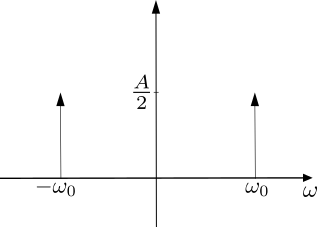
\includegraphics[width=.30\textwidth]{img/sine_spectrum.png} &
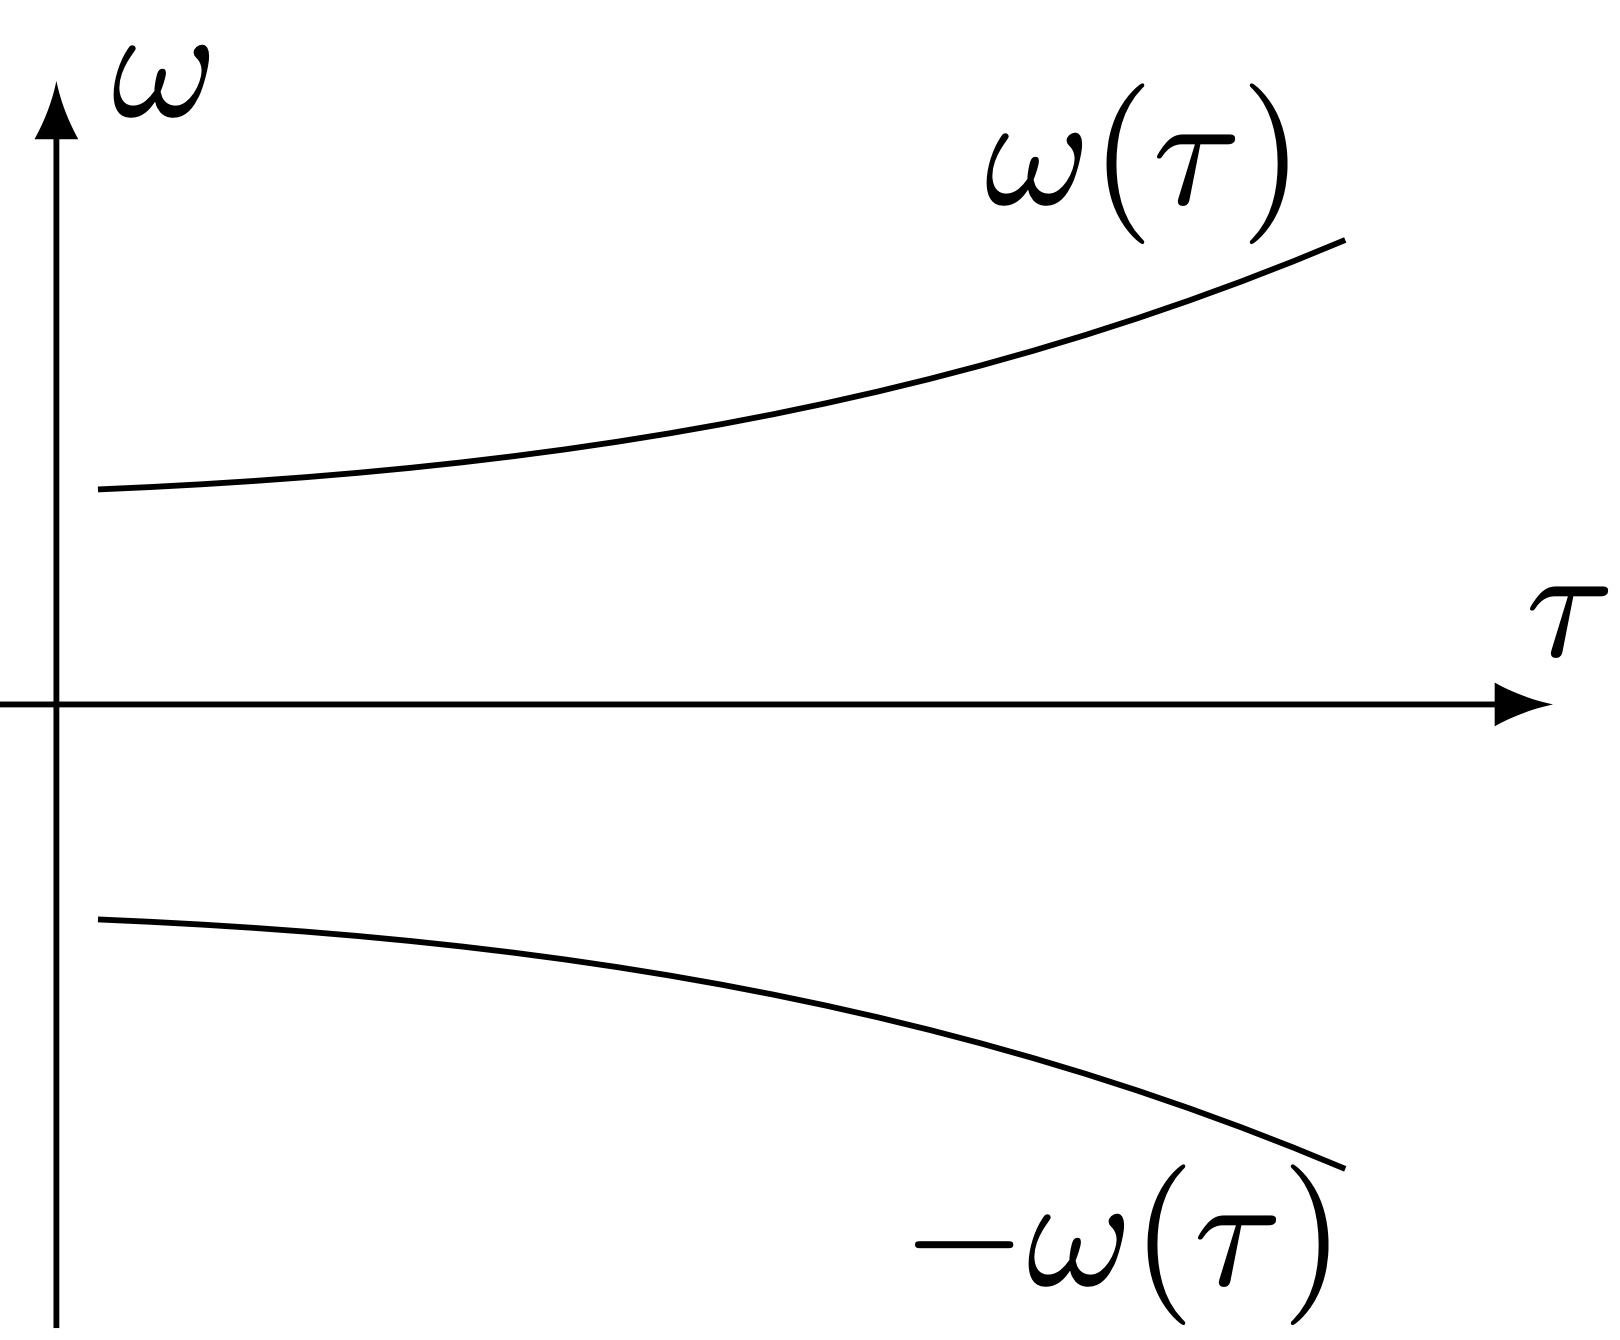
\includegraphics[width=.25\textwidth]{img/single_freq.png}\\[0.4em]
\end{tabular}

\end{frame}

\begin{frame}{The sound chirpiness - single time-varying frequency}
\protect\hypertarget{the-sound-chirpiness---single-time-varying-frequency}{}

\begin{columns}[T]
\begin{column}{0.7\textwidth}
Parametric representation of the sound \[s(t)=A\cdot sin(\w(t) t)\]

\begin{itemize}
\tightlist
\item
  In the time-frequency domain: \(t\mapsto(t,\w(t))\)
\item
  In the \emph{augmented space}: \(t\mapsto(t,\w(t),\nu(t))\)
\end{itemize}

with \[\nu(t)=\frac{\dw}{\dt}(t)\]
\end{column}

\begin{column}{0.3\textwidth}
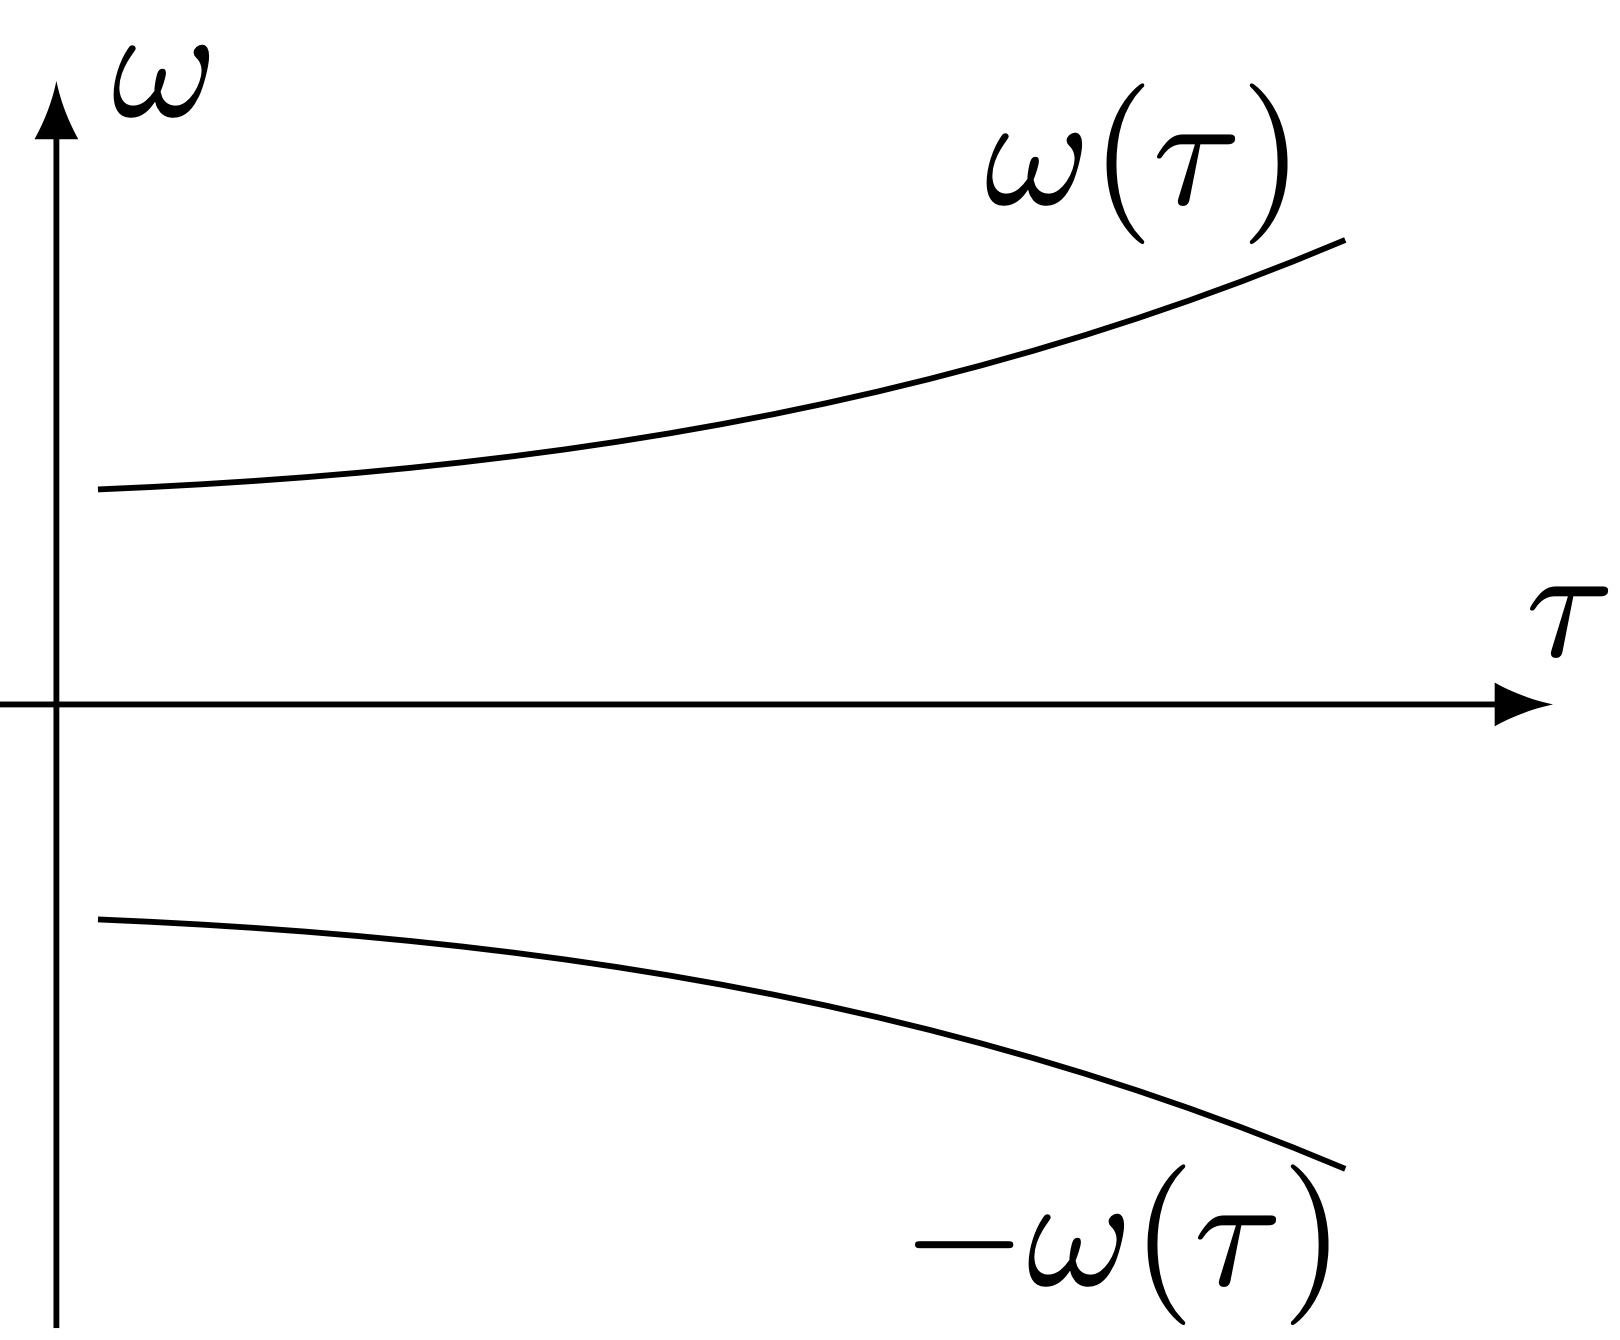
\includegraphics[width=1\textwidth,height=\textheight]{img/single_freq.png}
\end{column}
\end{columns}

\end{frame}

\begin{frame}{Representation in contact space - control system}
\protect\hypertarget{representation-in-contact-space---control-system}{}

What's the nature of the curve \(t\mapsto(t,\w(t),\nu(t))\)?

Let's define \(u(t)=\dnu/\dt\), the curve in the contact space
\(t\mapsto(t,\w(t),\nu(t))\) is \emph{a lift of a planar curve if there
exists a function} \(u(t)\) such that

\[\ddt\pmat{\tau\\\w\\\nu} = \pmat{1\\\nu\\0} + u(t)\pmat{0\\0\\1}\]

Let \(q=(\tau,\w,\nu)\), the previous equations is the state equation of
a control system written as \[\ddt q(t) = X_0(q(t)) + u(t) X_1(q(t))\]

where \(X_0(q(t))\) and \(X_1(q(t))\) are two vector fields in \(\R^3\)
\[X_0\pmat{\tau\\\w\\\nu} = \pmat{1\\\nu\\0},\quad 
X_1\pmat{\tau\\\w\\\nu} = \pmat{0\\0\\1}\]

\end{frame}

\begin{frame}{Representation in contact space - Heisenberg group}
\protect\hypertarget{representation-in-contact-space---heisenberg-group}{}

The two vector fields in \(\R^3\)
\[X_0\pmat{\tau\\\w\\\nu} = \pmat{1\\\nu\\0},\quad 
X_1\pmat{\tau\\\w\\\nu} = \pmat{0\\0\\1}\]

Generate the \textbf{Heisenberg group} because
{[}\protect\hyperlink{ref-boscain2021}{4},\protect\hyperlink{ref-grochenig2001}{11}{]}

\begin{itemize}
\tightlist
\item
  \(Z=[X_0,X_1]\neq 0\)
\item
  \([Z,X_0]=[Z,X_1]=0\)
\end{itemize}

\end{frame}

\begin{frame}{Lift to the contact space}
\protect\hypertarget{lift-to-the-contact-space}{}

We lift the each level line of the spectrum \(\abs{S}(\tau,\w)\) to the
contact space. Yeilding the following subset of the contact space, which
is a well-defined surface if \(\abs{S}\in\Cl^2\) and
\(\mathrm{Hess}\abs{S}\) is non-degenerate
{[}\protect\hyperlink{ref-boscain2021}{4}{]}.

\[\Sigma = \sset{(\tau,\w,\nu)\in\R^3 \vert\nu\partial_\w\abs{S}(\tau,\w) + \partial_\tau\abs{S}(\tau,\w) = 0}\]

Which allows to finally define the sound lift in the contact space as

\[L(\tau,\w,\nu) = S(\tau,\w)\cdot\delta_\Sigma (\tau,\w,\nu) =
\begin{cases}
S(\tau,\w) & \text{if}~(\tau,\w,\nu)\in\Sigma\\
0          & \text{otherwise}
\end{cases}\]

The time-frequency representation is obtained from the lifted sound by
applying the projection operator defined as

\[\Proj\sset{L(\tau,\w,\nu)}(\tau,\w) = \int_\R L(\tau,\w,\nu)\dnu\]

\end{frame}

\hypertarget{cortical-activations-in-a1}{%
\subsection{Cortical activations in
A1}\label{cortical-activations-in-a1}}

\begin{frame}{Cortical activations in A1 - Wilson-Cowan model}
\protect\hypertarget{cortical-activations-in-a1---wilson-cowan-model}{}

We model the cortical activations in A1 as follows

\begin{itemize}
\tightlist
\item
  The primary aidtory cortex (A1) is a space of \((\w,\nu)\in\R^2\).
\item
  A1 receives the sound lift to the contact space \(L(t,\w,\nu)\) at
  every instant \(t\).
\item
  The \emph{neuron} receives an external charge \(S(t,\w)\) if
  \((t,\w,\nu)\in\Sigma\) and no charge otherwise.
\end{itemize}

We need to model these neural activations \(\rightsquigarrow\)
Wilson-Cowan model

\begin{itemize}
\tightlist
\item
  Successfully applied to describe neural activations in V1 and A1
  {[}\protect\hyperlink{ref-bertalmio2018}{2},\protect\hyperlink{ref-boscain2017}{3},\protect\hyperlink{ref-bressloff2002a}{6},\protect\hyperlink{ref-ermentrout1979}{9},\protect\hyperlink{ref-loebel2007}{14},\protect\hyperlink{ref-rankin2015}{17},\protect\hyperlink{ref-zulfiqar2019}{21}{]}
\item
  Flexible model, applies independently to the underlying geometric
  structure
\item
  Geometric structure is encoded in the kernel of the integral term
\item
  Implementation of delay terms
\end{itemize}

\end{frame}

\begin{frame}{Wilson-Cowan equation}
\protect\hypertarget{wilson-cowan-equation}{}

\[\dtfrac a(t,\w,\nu) = -\alpha a(t,\w,\nu) + \beta L(t,\w,\nu)
+ \gamma\int_{\R^2} k_\delta(\w,\nu\Vert\w',\nu') \sigma(a(t-\delta,\w',\nu')) \dw'\dnu'\]

where

\begin{itemize}
\tightlist
\item
  \(\alpha,\beta,\gamma>0\) are (tuning) parameters
\item
  \(\sigma:\C\rightarrow\C\) is a non-linear sigmoid

  \begin{itemize}
  \tightlist
  \item
    \(\sigma(\rho e^{i\theta})=\tilde\sigma(\rho)e^{i\theta}\)
  \item
    \(\tilde\sigma(x)=\min\sset{\max\sset{0,\kappa x}, 1},\forall x\in\R\)
    given a fixed \(\kappa>0\)
  \end{itemize}
\item
  \(k_\delta(\w,\nu\Vert\w',\nu')\) is a weight modeling the interaction
  between \((\w,\nu)\) and \((\w',\nu')\) after a delay \(\delta>0\) via
  the kernel of the transport-diffusion operator associated to the
  contact structure of A1
\end{itemize}

\end{frame}

\begin{frame}{Wilson-Cowan equation with no delay}
\protect\hypertarget{wilson-cowan-equation-with-no-delay}{}

When \(\gamma=0\), the WC equation becomes a standard low-pass filter
\[\partial_t a(t,\w,\nu)=-\alpha a(t,\w,\nu) + L(t,\w,\nu)\]

whose solution is simply
\[a(t,\w,\nu) = \int_0^t e^{-\alpha(s-t)}L(t,\w,\nu)\ds\]

Here, \(\w\) and \(\nu\) are parameters \(\rightsquigarrow\) there is no
interaction between regions sensitive to different \(\w\) and \(\nu\).

\end{frame}

\begin{frame}{Wilson-Cowan equation with delayed interaction}
\protect\hypertarget{wilson-cowan-equation-with-delayed-interaction}{}

\[\dtfrac a(t,\w,\nu) = -\alpha a(t,\w,\nu) + \beta L(t,\w,\nu)
+ \gamma\int_{\R^2} k_\delta(\w,\nu\Vert\w',\nu') \sigma(a(t-\delta,\w',\nu')) \dw'\dnu'\]

With \(\gamma\neq0\), a non-linear term is added on top of the low-pass
filter:

\begin{itemize}
\tightlist
\item
  The added term describes the diffusion of the activation in side A1
\item
  The added term encodes the inhibitory and excitatory interconnections
  between neurons
\item
  The sigmoid is a non-linear function that saturates the signal \(a\)
\end{itemize}

\end{frame}

\hypertarget{implementation}{%
\section{Implementation}\label{implementation}}

\hypertarget{the-wca1.jl-package}{%
\subsection{\texorpdfstring{The \texttt{WCA1.jl}
package}{The WCA1.jl package}}\label{the-wca1.jl-package}}

\begin{frame}{The Julia language}
\protect\hypertarget{the-julia-language}{}

The Julia language is

\begin{itemize}
\tightlist
\item
  New

  \begin{itemize}
  \tightlist
  \item
    First appeared in 2012
  \item
    Version 1.0 was released in 2018
  \end{itemize}
\item
  Fast: comparable to Fortran and C
\item
  Easy to use: similar to Python, Matlab, and R
\item
  General-purpose
\item
  Great for scientific computing
\end{itemize}

Julia community is small: in 2021 Stack Overflow Developer Survey
{[}\protect\hyperlink{ref-so_survey2021}{22}{]} ``Which language
developers wanted to work in over the next year?''

\begin{itemize}
\tightlist
\item
  Julia: 1.29\%
\item
  Python: 48.24\%
\item
  Matlab: 4.66\%
\end{itemize}

Result: less stable scientific libraries in Julia than other languages

\end{frame}

\begin{frame}[fragile]{The \texttt{WCA1.jl} package}
\protect\hypertarget{the-wca1.jl-package-1}{}

\begin{itemize}
\tightlist
\item
  Original code:
  \href{https://github.com/dprn/WCA1}{\texttt{https://github.com/dprn/WCA1}}
\item
  Forked repository:
  \href{https://github.com/rand-asswad/WCA1}{\texttt{https://github.com/rand-asswad/WCA1}}
\end{itemize}


\includegraphics{img/github_contributions.png}

Issues with original code:

\begin{itemize}
\tightlist
\item
  Unstable \(\rightsquigarrow\) failed to run on speech signals
\item
  Far from optimal \(\rightsquigarrow\) took long time to run on speech
  signals
\item
  Low readability
\item
  Non-conforming to Julia's code norms and performance recommendations
\end{itemize}

\end{frame}

\begin{frame}[fragile]{The STFT module}
\protect\hypertarget{the-stft-module}{}

\textbf{Issue:} no implementation of the inverse STFT in Julia's
standard libraries
(\href{https://juliapackages.com/p/fftw}{\texttt{FFTW.jl}}
and\href{https://juliapackages.com/p/dsp}{\texttt{DSP.jl}}).

\textbf{Solution:} implemented the Griffin-Lim algorithm
{[}\protect\hyperlink{ref-griffin1983}{10}{]} from scratch

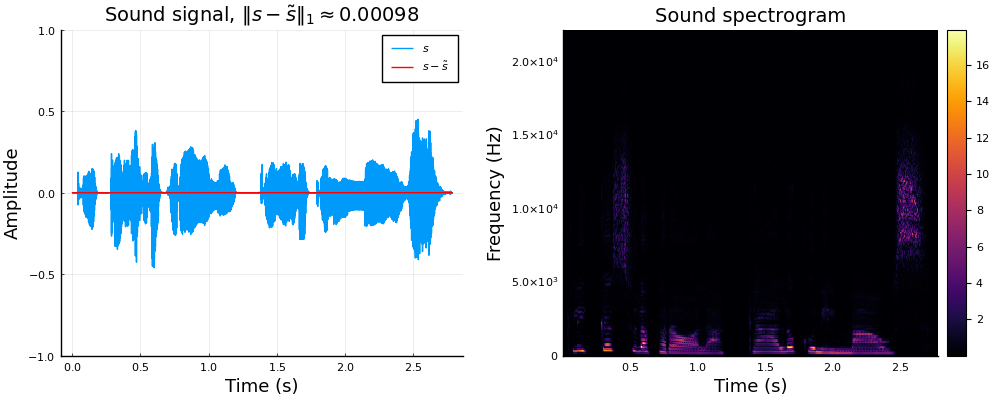
\includegraphics{img/stft_istft.png}

\end{frame}

\begin{frame}{The Lift module - calculating chirpiness values}
\protect\hypertarget{the-lift-module---calculating-chirpiness-values}{}

The sound chirpiness is defined as
\[\nu\partial_\omega\abs{S}(\tau,\omega) + \partial_\tau\abs{S}(\tau,\omega)=0\]

We compute the chirpiness with respect to each time-frequency pair by
calculating the gradient of the spectrum \(\nabla\abs{S}\).

\[\nu(\tau,\w) =
\begin{cases}
-\frac{\partial_\tau\abs{S}(\tau,\w)}{\partial_\w\abs{S}(\tau,\w)} & \text{if}~\abs{\partial_\w\abs{S}(\tau,\w)}>\epsilon\\
0 & \text{otherwise}
\end{cases}\]

where \(\epsilon\) is a small threshold.

\end{frame}

\begin{frame}{The Lift module - chirpiness sampling issue}
\protect\hypertarget{the-lift-module---chirpiness-sampling-issue}{}

\textbf{Issue:} the chipriness values \(\nu\) are unbounded since
\[\nu\partial_\omega\abs{S}(\tau,\omega) + \partial_\tau\abs{S}(\tau,\omega)=0\]

and there exists points \((\tau_0,\w_0)\) such that
\(\partial_\omega\abs{S}(\tau_0,\omega_0)=0\)

therefore chirpiness values stretch over the entire real line (coverge
to \(\pm\infty\))

\textbf{Original solution:} manually restrict chirpiness values to
\(\nu\in[\numin,\numax]\) for synthetic signals (the limits are
determined after visualizing the histogram of the chirpiness values).

\textbf{Needed solution:} a reliable method to automatically determine
the interval \([\numin,\numax]\) without losing (a lot of) values.

\end{frame}

\begin{frame}{The Lift module - chirpiness values distribution}
\protect\hypertarget{the-lift-module---chirpiness-values-distribution}{}

We noticed that the chirpiness values of speech signals follow a Cauchy
distribution {[}\protect\hyperlink{ref-asswad2021}{1}{]}

\begin{columns}[T]
\begin{column}{0.6\textwidth}
Let \(X\) be a random variable following \(\Cd(x_0, \gamma)\)

\begin{itemize}
\tightlist
\item
  \textbf{Location parameter \(x_0\):} location of the peak
\item
  \textbf{Scale parameter \(\gamma\):} half the interquartile range
\end{itemize}

Probability density function (PDF):
\[f_X(x)=\frac{1}{\pi\gamma\pp{1+\pp{\frac{x-x_0}{\gamma}}^2}}\]

Cumulative distribution function (CDF):
\[F_X(x)=\frac{1}{\pi} \arctan\pp{\frac{x-x_0}{\gamma}} + \frac{1}{2}\]
\end{column}

\begin{column}{0.4\textwidth}
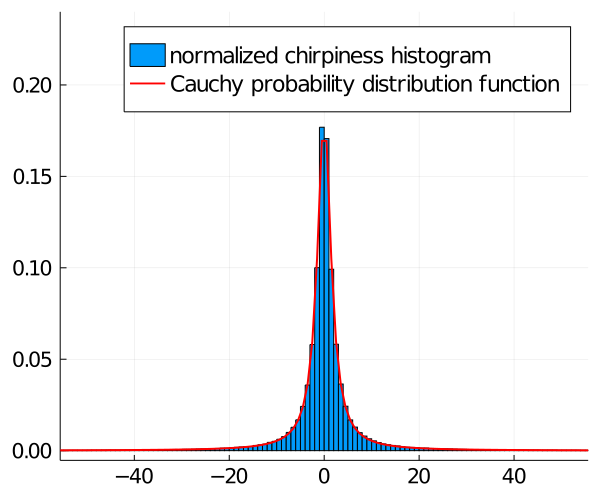
\includegraphics{img/cauchy_dist_pdf.png}
\end{column}
\end{columns}

\end{frame}

\begin{frame}{The Lift module - chirpiness values distribution}
\protect\hypertarget{the-lift-module---chirpiness-values-distribution-1}{}

\begin{columns}[T]
\begin{column}{0.5\textwidth}
Estimating Cauchy parameters \(\Cd(x_0, \gamma)\):

\begin{itemize}
\tightlist
\item
  \(x_0\): the chirpiness samples median
\item
  \(\gamma\): half the interquartile range (difference between the
  75\textsuperscript{th} and the 25\textsuperscript{th} percentile)
\end{itemize}

Assumption: \[\nu\sim\Cd\pp{\med(\nu),\frac{Q(75\%)-Q(25\%)}{2}}\]

Stastical tests on a library of real speech signals \textbf{rejected}
the assumption.

Nevertheless, the fit is quite good according to the Kolomogorov-Smirnov
statistic \[D_n=\sup_x\abs{F_n(x)-F_X(x)}\]

where \(F_n\) is the empirical distribution function
\end{column}

\begin{column}{0.5\textwidth}
\begin{center}\centering
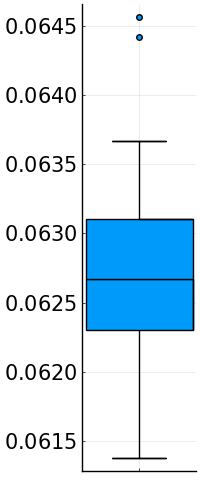
\includegraphics[width=0.3\textwidth]{img/cauchy_pt_estimate_iqr_2.png}
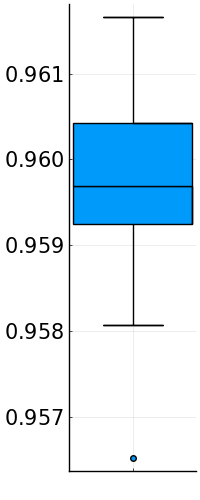
\includegraphics[width=0.3\textwidth]{img/cauchy_values_percentage_iqr_2.png}
\end{center}

Box plots for estimated Cauchy distributions of speech signals
chirpiness values

\begin{itemize}
\tightlist
\item
  \emph{left:} Kolmogorov-Smirnov statistic values.
\item
  \emph{right:} percentage of values falling in \(I_{0.95}\)
\end{itemize}
\end{column}
\end{columns}

\end{frame}

\begin{frame}{The Lift module - chirpiness sampling}
\protect\hypertarget{the-lift-module---chirpiness-sampling}{}

\begin{enumerate}
\tightlist
\item
  Calculate chirpiness values for each \((\tau,\w)\)
\item
  Compute values to Cauchy distribution to find confidence interval
  \(I_p=[\numin,\numax]\)
\item
  Discretize chirpiness values \(\nu\in I_p\) as follows
\end{enumerate}

Let \((\nu_n)_{1\leq n\leq N}\) such that
\(\numin=\nu_1<\cdots<\nu_N=\numax\).

Each value \(\nu\) is rounded to the nearest \(\nu_n\).

\[n(\nu) = \round{\frac{\nu - \numin}{\numax - \numin}(N-1) + 1},\quad\forall\nu\in I_p\]

where \(\round{\cdot}:\R\rightarrow\Z\) is the rounding function to the
nearest integer.

\end{frame}

\begin{frame}{The Lift module - chirpiness sampling optimization}
\protect\hypertarget{the-lift-module---chirpiness-sampling-optimization}{}

The function \(n(\nu)\) can be optimized by rewriting it as an affine
function

\[n(\nu) = \round{\frac{\nu - \numin}{\numax - \numin}(N-1) + 1}
  = \round{\underbrace{\pp{\frac{N-1}{\numax - \numin}}}_a \cdot\nu
    + \underbrace{\pp{1 - \frac{(N-1)\numin}{\numax - \numin}}}_b}
  = \round{a\cdot\nu + b}\]

This reduces the number of arithmetic operations inside the loop in
\(O(n)\) complexity.

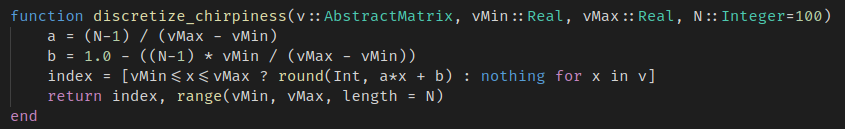
\includegraphics{img/chirpiness_function.png}

\end{frame}

\begin{frame}{The Lift module - chirpiness sampling benchmark}
\protect\hypertarget{the-lift-module---chirpiness-sampling-benchmark}{}

Using Julia's standard benchmark tools, we ran a benchmark on the speech
library samples with different chirpiness implementations.

\begin{columns}[T]
\begin{column}{0.6\textwidth}
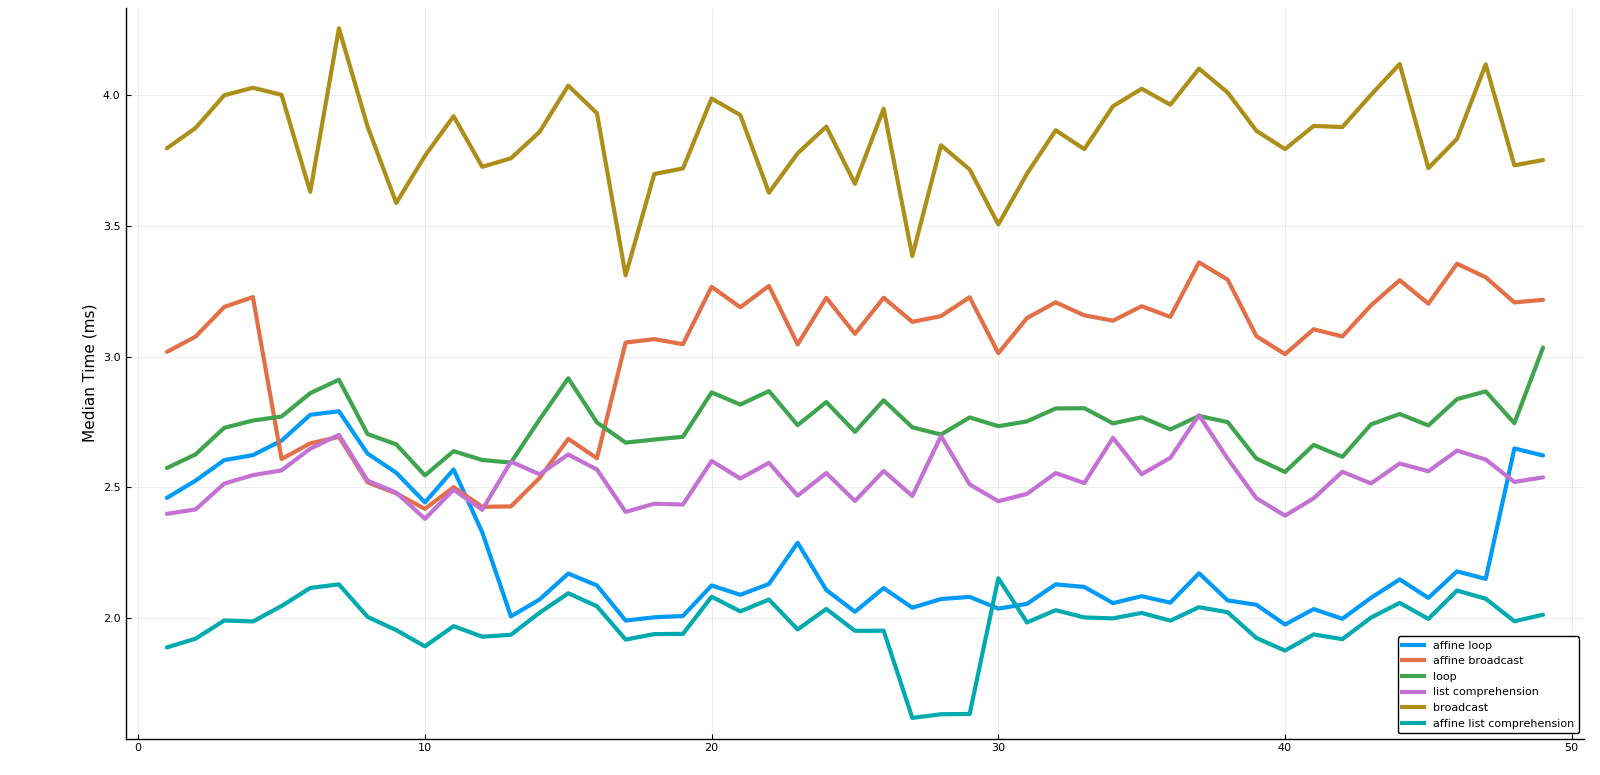
\includegraphics[width=1\textwidth,height=\textheight]{img/benchmark_median_time.png}

The benchmarked median time for each method ploted against the speech
samples
\end{column}

\begin{column}{0.4\textwidth}
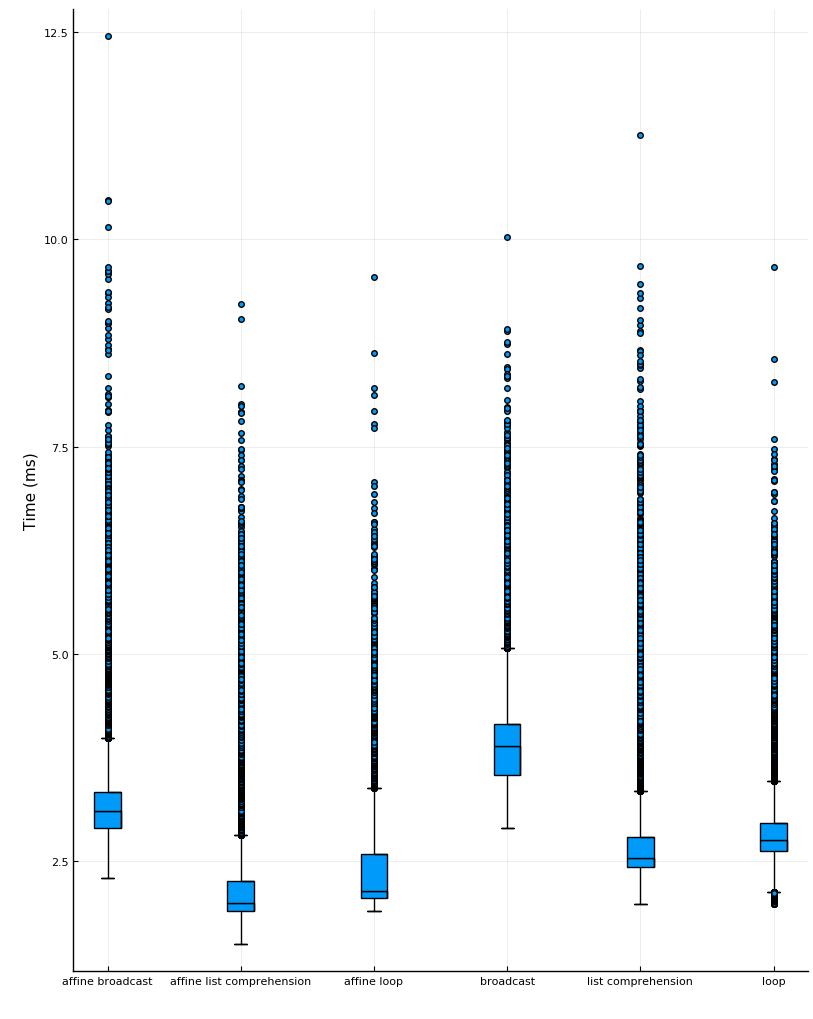
\includegraphics[width=0.8\textwidth,height=\textheight]{img/benchmark_time_boxplot.png}

Box plots of the benchmarked time for each method on the samples from
the speech library
\end{column}
\end{columns}

\end{frame}

\hypertarget{published-results}{%
\subsection{Published results}\label{published-results}}

\begin{frame}{Denoising experiment
{[}\protect\hyperlink{ref-asswad2021}{1}{]}}
\protect\hypertarget{denoising-experiment-asswad2021}{}

We apply a gaussian random noise \(g_\eps\sim\Nd(0,\eps)\) to a an input
sound \(s\), we process the noisy sound input through the algorithm
pipeline

\begin{itemize}
\tightlist
\item
  \textbf{Input:} \(s_\eps = s + g_\eps\)
\item
  \textbf{Output:}
  \(\tilde s_\eps=\STFT^{-1}\circ\Proj\circ\mathrm{WC}\circ\mathrm{Lift}\circ\STFT(s_\eps)\)
\end{itemize}

\begin{columns}[T]
\begin{column}{0.5\textwidth}
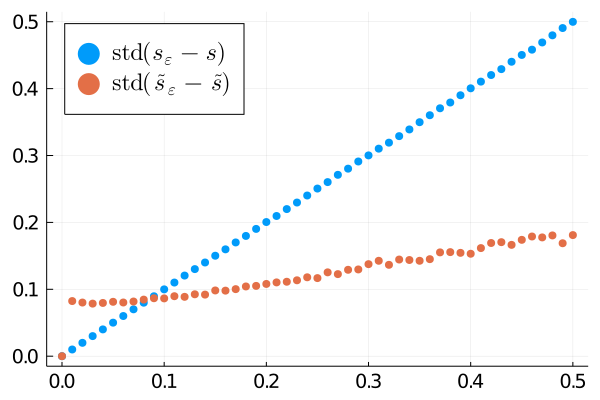
\includegraphics[width=0.9\textwidth,height=\textheight]{img/std_diff.png}
\end{column}

\begin{column}{0.5\textwidth}
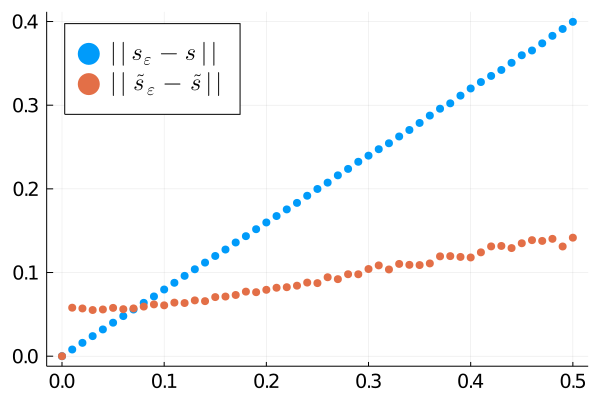
\includegraphics[width=0.9\textwidth,height=\textheight]{img/norm_diff.png}
\end{column}
\end{columns}

Distance of noisy sound to original one before (blue) and after (red)
the processing, plotted against the standard deviation of the noise
\(\eps\) (where \(\norm{s}=\norm{s}_1/\dim(s)\))

\end{frame}

\hypertarget{conclusion}{%
\section{Conclusion}\label{conclusion}}

\hypertarget{reviewing-the-model}{%
\subsection{Reviewing the model}\label{reviewing-the-model}}

\begin{frame}{Model analysis}
\protect\hypertarget{model-analysis}{}

The sound reconstruction model:

\begin{itemize}
\tightlist
\item
  improves noisy speech signals
\item
  is mathematically stable
\item
  has great potential
\end{itemize}

Conclusion:

\begin{itemize}
\tightlist
\item
  the model should be improved and adapted to more corrupted sounds
\item
  the model deserves to be the basis of a PhD project
\end{itemize}

We will see the paths we explored to improve the model

\end{frame}

\begin{frame}{Model analysis - Lift drawbacks}
\protect\hypertarget{model-analysis---lift-drawbacks}{}

\begin{columns}[T]
\begin{column}{0.5\textwidth}
\begin{itemize}
\tightlist
\item
  The lifted representation
  \(L(\tau,\w,\nu)=S(\tau,\w)\delta_\sigma(\tau,\w,\nu)\) depends on the
  phase of \(S(\tau,\w)\in\C\). This is unrealistic, since the cochlea
  only transmits the spectrogram \(\abs{S(\tau,\w)}\) because A1 is
  insensitive to phase.
\item
  At a fixed time \(t>0\), the resulting representation \(L(t,\w,\nu)\)
  is a distribution, concentrated on a one dimensional curve in the
  frequency-chirpiness space which is also unrealistic.
\item
  The current procedure to obtain \(L(\tau,\w,\nu)\) requires to first
  compute \(S(\tau,\w)\) and then to ``lift'' it. We would like to
  obtain \(L\) directly from the original signal \(s\).
\end{itemize}
\end{column}

\begin{column}{0.5\textwidth}
To improve the model, it is crucial to devise a novel lift procedure
allowing to bypass these problems.

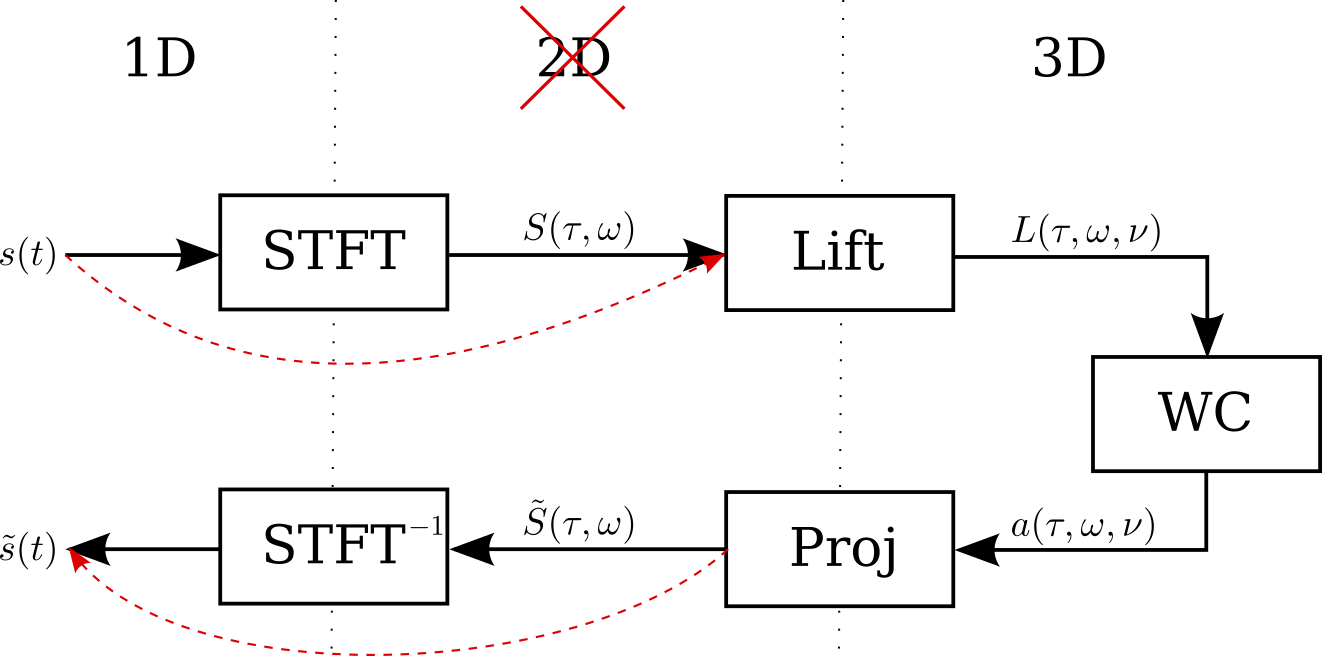
\includegraphics[width=1\textwidth,height=\textheight]{img/new_pipeline.png}

Alternative sound reconstruction pipeline
\end{column}
\end{columns}

\end{frame}

\begin{frame}{Model analysis - Wavelet Transform}
\protect\hypertarget{model-analysis---wavelet-transform}{}

By reading state-of-the-art literature on the neurophysiology of the
inner ear, we realized that a Wavelet transform represents the signal
processing in the cochlea than the STFT transform
{[}\protect\hyperlink{ref-reimann2011}{18},\protect\hyperlink{ref-yang1992}{20}{]}.

\begin{definition}[Wavelet Transform]
The Wavelet Transform (WT) of a realizable signal $s\in L^2(\R)$ along
a wavelet $\psi\in L^2(\R)$ is defined by
$$W_\psi s(a,t) = \frac{1}{\sqrt{a}} \int_\R s(\tau) \overline{\psi\pp{\frac{\tau-t}{a}}} \dtau$$
where $a$ is the dilation variable.
\end{definition}

\end{frame}

\begin{frame}{Model analysis - Wavelet Transform}
\protect\hypertarget{model-analysis---wavelet-transform-1}{}

\textbf{Advantage:} time resolution increases for higher frequencies in
the WT.

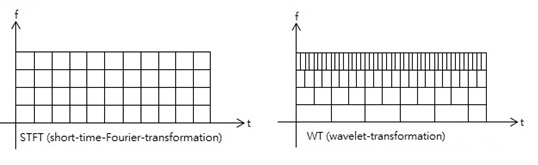
\includegraphics{img/stft_vs_wt.jpg}

\textbf{Disadvantage:} the dilation variable \(a\) implicitly represents
the frequency \(\w\).

\begin{itemize}
\tightlist
\item
  Obtaining the sound chirpiness \(\nu\) is not straightforward as in
  the case of the STFT
\item
  We haven't been able to define an appropriate lift from the WT
\end{itemize}

\end{frame}

\begin{frame}{Model analysis - the lift operator}
\protect\hypertarget{model-analysis---the-lift-operator}{}

We defined the STFT as operator on \(L^2(\R)\) in function of the
unitary shift operators

\[V_w s(\tau,\w) = \dotp{s, M_\w T_\tau w}_{L^2(\R)}\]

We would like to have

\[L_\gamma s(\tau,\w,\nu) = \dotp{s,C_\nu M_\w T_\tau \gamma}_{L^2(\R)}\]

where \(C_\nu\in\U(L^2(\R))\)

Such operator would be

\begin{itemize}
\tightlist
\item
  Mathematically stable and elegant
\item
  Computationally cheap
\end{itemize}

\end{frame}

\hypertarget{acquired-knowledge}{%
\subsection{Acquired knowledge}\label{acquired-knowledge}}

\begin{frame}{Acquired knowledge}
\protect\hypertarget{acquired-knowledge-1}{}

\begin{itemize}
\tightlist
\item
  Fundamental mathematics

  \begin{itemize}
  \tightlist
  \item
    Geometry
  \item
    Group representations
  \item
    Operator algebra
  \item
    Time-Frequency analysis
  \end{itemize}
\item
  Applied mathematics \& programming

  \begin{itemize}
  \tightlist
  \item
    Signal processing \& DSP
  \item
    Julia language
  \item
    Neural activations models
  \end{itemize}
\item
  The neuro-physiology of the inner ear
\item
  Research experience

  \begin{itemize}
  \tightlist
  \item
    Studying state-of-the-art litterature
  \item
    Co-writing a conference paper
  \item
    Attending the GSI 2021 conference
  \end{itemize}
\end{itemize}

\end{frame}

\hypertarget{future-project}{%
\subsection{Future project}\label{future-project}}

\begin{frame}{My future project}
\protect\hypertarget{my-future-project}{}

After my internship, I have decided to pursue

\begin{itemize}
\tightlist
\item
  a Master's degree in fundamental mathematics at Université de
  Lorraine, focusing on PDEs and Control Theory
\item
  a PhD thesis in the domains of PDEs and Control Theory
\item
  a career in academic research
\end{itemize}

\end{frame}

\begin{frame}

\centering

\huge Thank you for your attention!

\end{frame}

\hypertarget{references}{%
\subsection{References}\label{references}}

\begin{frame}[allowframebreaks]{References}
\protect\hypertarget{references-1}{}

\hypertarget{refs}{}
\leavevmode\hypertarget{ref-asswad2021}{}%
{[}1{]} Rand Asswad, Ugo Boscain, Giuseppina Turco, Dario Prandi, and
Ludovic Sacchelli. 2021. An Auditory Cortex Model for Sound Processing..
56--64. DOI:\url{https://doi.org/10.1007/978-3-030-80209-7_7}

\leavevmode\hypertarget{ref-bertalmio2018}{}%
{[}2{]} Marcelo Bertalmío, Luca Calatroni, Valentina Franceschi,
Benedetta Franceschiello, and Dario Prandi. 2018. A cortical-inspired
model for orientation-dependent contrast perception: A link with
Wilson-Cowan equations. \emph{arXiv:1812.07425 {[}cs{]}} (December
2018). Retrieved November 12, 2020 from
\url{http://arxiv.org/abs/1812.07425}

\leavevmode\hypertarget{ref-boscain2017}{}%
{[}3{]} Ugo Boscain, Roman Chertovskih, Jean-Paul Gauthier, Dario
Prandi, and Alexey Remizov. 2017. Cortical-inspired image reconstruction
via sub-Riemannian geometry and hypoelliptic diffusion. In \emph{SMAI
2017 - 8e Biennale Française des Mathématiques Appliquées et
Industrielles}, La Tremblade, France, 37--53.
DOI:\url{https://doi.org/10.1051/proc/201864037}

\leavevmode\hypertarget{ref-boscain2021}{}%
{[}4{]} Ugo Boscain, Dario Prandi, Ludovic Sacchelli, and Giuseppina
Turco. 2021. A bio-inspired geometric model for sound reconstruction.
\emph{The Journal of Mathematical Neuroscience} 11, 1 (January 2021), 2.
DOI:\url{https://doi.org/10.1186/s13408-020-00099-4}

\leavevmode\hypertarget{ref-bressloff2002}{}%
{[}5{]} Paul C. Bressloff and Jack D. Cowan. 2002. An Amplitude Equation
Approach to Contextual Effects in Visual Cortex. \emph{Neural
Computation} 14, 3 (March 2002), 493--525.
DOI:\url{https://doi.org/10.1162/089976602317250870}

\leavevmode\hypertarget{ref-bressloff2002a}{}%
{[}6{]} Paul C. Bressloff, Jack D. Cowan, Martin Golubitsky, Peter J.
Thomas, and Matthew C. Wiener. 2002. What Geometric Visual
Hallucinations Tell Us about the Visual Cortex. \emph{Neural
Computation} 14, 3 (March 2002), 473--491.
DOI:\url{https://doi.org/10.1162/089976602317250861}

\leavevmode\hypertarget{ref-citti2006}{}%
{[}7{]} G. Citti and A. Sarti. 2006. A Cortical Based Model of
Perceptual Completion in the Roto-Translation Space. \emph{Journal of
Mathematical Imaging and Vision} 24, 3 (May 2006), 307--326.
DOI:\url{https://doi.org/10.1007/s10851-005-3630-2}

\leavevmode\hypertarget{ref-dallos1996}{}%
{[}8{]} P. Dallos. 1996. Overview: Cochlear Neurobiology: Springer
Handbook of Auditory Research. \emph{The Cochlea: Springer Handbook of
Auditory Research} (1996), 1--43. Retrieved August 13, 2021 from
\url{https://www.scholars.northwestern.edu/en/publications/overview-cochlear-neurobiology-springer-handbook-of-auditory-rese}

\leavevmode\hypertarget{ref-ermentrout1979}{}%
{[}9{]} G. B. Ermentrout and J. D. Cowan. 1979. A mathematical theory of
visual hallucination patterns. \emph{Biological Cybernetics} 34, 3
(October 1979), 137--150. DOI:\url{https://doi.org/10.1007/BF00336965}

\leavevmode\hypertarget{ref-griffin1983}{}%
{[}10{]} D. Griffin and Jae S. Lim. 1983. Signal estimation from
modified short-time Fourier transform. \emph{undefined} (1983).
Retrieved September 3, 2021 from
\url{https://www.semanticscholar.org/paper/Signal-estimation-from-modified-short-time-Fourier-Griffin-Lim/14bc876fae55faf5669beb01667a4f3bd324a4f1}

\leavevmode\hypertarget{ref-grochenig2001}{}%
{[}11{]} Karlheinz Gröchenig. 2001. \emph{Foundations of Time-Frequency
Analysis}. Birkhäuser Basel.
DOI:\url{https://doi.org/10.1007/978-1-4612-0003-1}

\leavevmode\hypertarget{ref-hoffman1989}{}%
{[}12{]} William C. Hoffman. 1989. The visual cortex is a contact
bundle. \emph{Applied Mathematics and Computation} 32, 2 (August 1989),
137--167. DOI:\url{https://doi.org/10.1016/0096-3003(89)90091-X}

\leavevmode\hypertarget{ref-hubel1959}{}%
{[}13{]} D. H. Hubel and T. N. Wiesel. 1959. Receptive fields of single
neurones in the cat's striate cortex. \emph{The Journal of Physiology}
148, 3 (1959), 574--591.
DOI:\url{https://doi.org/10.1113/jphysiol.1959.sp006308}

\leavevmode\hypertarget{ref-loebel2007}{}%
{[}14{]} Alex Loebel, Israel Nelken, and Misha Tsodyks. 2007. Processing
of sounds by population spikes in a model of primary auditory cortex.
\emph{Frontiers in Neuroscience} 1, 1 (November 2007), 197--209.
DOI:\url{https://doi.org/10.3389/neuro.01.1.1.015.2007}

\leavevmode\hypertarget{ref-muller2015}{}%
{[}15{]} Meinard Müller. 2015. \emph{Fundamentals of Music Processing -
Audio, Analysis, Algorithms, Applications}. Springer. Retrieved from
\url{https://www.audiolabs-erlangen.de/fau/professor/mueller/bookFMP}

\leavevmode\hypertarget{ref-petitot1999}{}%
{[}16{]} Jean Petitot and Yannick Tondut. 1999. Vers une neurogéométrie.
Fibrations corticales, structures de contact et contours subjectifs
modaux. \emph{Mathématiques et Sciences Humaines} 145, (1999), 5--101.
Retrieved August 13, 2021 from \url{https://eudml.org/doc/94522}

\leavevmode\hypertarget{ref-rankin2015}{}%
{[}17{]} James Rankin, Elyse Sussman, and John Rinzel. 2015.
Neuromechanistic Model of Auditory Bistability. \emph{PLoS computational
biology} 11, 11 (November 2015), e1004555.
DOI:\url{https://doi.org/10.1371/journal.pcbi.1004555}

\leavevmode\hypertarget{ref-reimann2011}{}%
{[}18{]} Hans Martin Reimann. 2011. Signal processing in the cochlea:
The structure equations. \emph{The Journal of Mathematical Neuroscience}
1, 1 (June 2011), 5. DOI:\url{https://doi.org/10.1186/2190-8567-1-5}

\leavevmode\hypertarget{ref-wilson1972}{}%
{[}19{]} Hugh R. Wilson and Jack D. Cowan. 1972. Excitatory and
Inhibitory Interactions in Localized Populations of Model Neurons.
\emph{Biophysical Journal} 12, 1 (January 1972), 1--24.
DOI:\url{https://doi.org/10.1016/S0006-3495(72)86068-5}

\leavevmode\hypertarget{ref-yang1992}{}%
{[}20{]} Xiaowei Yang, Kuansan Wang, and Shihab Shamma. 1992. Auditory
representations of acoustic signals. \emph{Information Theory, IEEE
Transactions on} 38, (April 1992), 824--839.
DOI:\url{https://doi.org/10.1109/18.119739}

\leavevmode\hypertarget{ref-zulfiqar2019}{}%
{[}21{]} Isma Zulfiqar, Michelle Moerel, and Elia Formisano. 2019.
Spectro-Temporal Processing in a Two-Stream Computational Model of
Auditory Cortex. \emph{Frontiers in Computational Neuroscience} 13,
(2019), 95. DOI:\url{https://doi.org/10.3389/fncom.2019.00095}

\leavevmode\hypertarget{ref-so_survey2021}{}%
{[}22{]} 2021. Stack Overflow Developer Survey 2021. Retrieved from
\url{https://insights.stackoverflow.com/survey/2021\#section-most-popular-technologies-programming-scripting-and-markup-languages}

\end{frame}

\end{document}
